% Created by tikzDevice version 0.12.6 on 2025-02-11 17:01:22
% !TEX encoding = UTF-8 Unicode
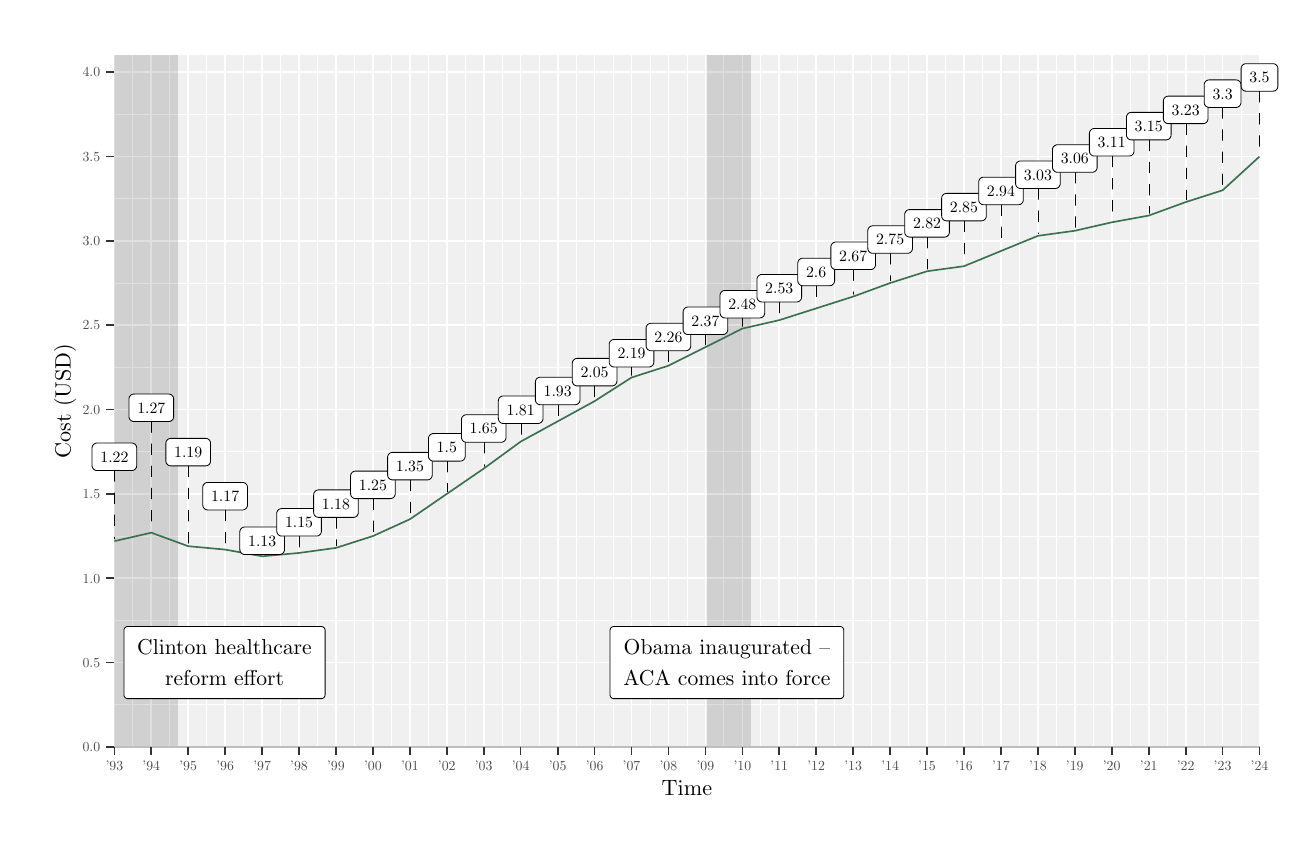
\begin{tikzpicture}[x=1pt,y=1pt]
\definecolor{fillColor}{RGB}{255,255,255}
\path[use as bounding box,fill=fillColor,fill opacity=0.00] (0,0) rectangle (455.30,289.08);
\begin{scope}
\path[clip] (  0.00,  0.00) rectangle (455.30,289.08);
\definecolor{drawColor}{RGB}{255,255,255}
\definecolor{fillColor}{RGB}{255,255,255}

\path[draw=drawColor,line width= 0.6pt,line join=round,line cap=round,fill=fillColor] (  0.00,  0.00) rectangle (455.30,289.08);
\end{scope}
\begin{scope}
\path[clip] (  0.00,  0.00) rectangle (455.30,289.08);
\definecolor{fillColor}{gray}{0.94}

\path[fill=fillColor] ( 31.15, 29.18) rectangle (445.30,279.08);
\definecolor{drawColor}{RGB}{255,255,255}

\path[draw=drawColor,line width= 0.3pt,line join=round] ( 31.15, 44.42) --
	(445.30, 44.42);

\path[draw=drawColor,line width= 0.3pt,line join=round] ( 31.15, 74.89) --
	(445.30, 74.89);

\path[draw=drawColor,line width= 0.3pt,line join=round] ( 31.15,105.37) --
	(445.30,105.37);

\path[draw=drawColor,line width= 0.3pt,line join=round] ( 31.15,135.84) --
	(445.30,135.84);

\path[draw=drawColor,line width= 0.3pt,line join=round] ( 31.15,166.32) --
	(445.30,166.32);

\path[draw=drawColor,line width= 0.3pt,line join=round] ( 31.15,196.80) --
	(445.30,196.80);

\path[draw=drawColor,line width= 0.3pt,line join=round] ( 31.15,227.27) --
	(445.30,227.27);

\path[draw=drawColor,line width= 0.3pt,line join=round] ( 31.15,257.75) --
	(445.30,257.75);

\path[draw=drawColor,line width= 0.3pt,line join=round] ( 38.00, 29.18) --
	( 38.00,279.08);

\path[draw=drawColor,line width= 0.3pt,line join=round] ( 51.34, 29.18) --
	( 51.34,279.08);

\path[draw=drawColor,line width= 0.3pt,line join=round] ( 64.68, 29.18) --
	( 64.68,279.08);

\path[draw=drawColor,line width= 0.3pt,line join=round] ( 78.04, 29.18) --
	( 78.04,279.08);

\path[draw=drawColor,line width= 0.3pt,line join=round] ( 91.40, 29.18) --
	( 91.40,279.08);

\path[draw=drawColor,line width= 0.3pt,line join=round] (104.74, 29.18) --
	(104.74,279.08);

\path[draw=drawColor,line width= 0.3pt,line join=round] (118.08, 29.18) --
	(118.08,279.08);

\path[draw=drawColor,line width= 0.3pt,line join=round] (131.44, 29.18) --
	(131.44,279.08);

\path[draw=drawColor,line width= 0.3pt,line join=round] (144.79, 29.18) --
	(144.79,279.08);

\path[draw=drawColor,line width= 0.3pt,line join=round] (158.13, 29.18) --
	(158.13,279.08);

\path[draw=drawColor,line width= 0.3pt,line join=round] (171.47, 29.18) --
	(171.47,279.08);

\path[draw=drawColor,line width= 0.3pt,line join=round] (184.83, 29.18) --
	(184.83,279.08);

\path[draw=drawColor,line width= 0.3pt,line join=round] (198.19, 29.18) --
	(198.19,279.08);

\path[draw=drawColor,line width= 0.3pt,line join=round] (211.53, 29.18) --
	(211.53,279.08);

\path[draw=drawColor,line width= 0.3pt,line join=round] (224.87, 29.18) --
	(224.87,279.08);

\path[draw=drawColor,line width= 0.3pt,line join=round] (238.23, 29.18) --
	(238.23,279.08);

\path[draw=drawColor,line width= 0.3pt,line join=round] (251.58, 29.18) --
	(251.58,279.08);

\path[draw=drawColor,line width= 0.3pt,line join=round] (264.92, 29.18) --
	(264.92,279.08);

\path[draw=drawColor,line width= 0.3pt,line join=round] (278.26, 29.18) --
	(278.26,279.08);

\path[draw=drawColor,line width= 0.3pt,line join=round] (291.62, 29.18) --
	(291.62,279.08);

\path[draw=drawColor,line width= 0.3pt,line join=round] (304.98, 29.18) --
	(304.98,279.08);

\path[draw=drawColor,line width= 0.3pt,line join=round] (318.32, 29.18) --
	(318.32,279.08);

\path[draw=drawColor,line width= 0.3pt,line join=round] (331.66, 29.18) --
	(331.66,279.08);

\path[draw=drawColor,line width= 0.3pt,line join=round] (345.02, 29.18) --
	(345.02,279.08);

\path[draw=drawColor,line width= 0.3pt,line join=round] (358.37, 29.18) --
	(358.37,279.08);

\path[draw=drawColor,line width= 0.3pt,line join=round] (371.71, 29.18) --
	(371.71,279.08);

\path[draw=drawColor,line width= 0.3pt,line join=round] (385.05, 29.18) --
	(385.05,279.08);

\path[draw=drawColor,line width= 0.3pt,line join=round] (398.41, 29.18) --
	(398.41,279.08);

\path[draw=drawColor,line width= 0.3pt,line join=round] (411.77, 29.18) --
	(411.77,279.08);

\path[draw=drawColor,line width= 0.3pt,line join=round] (425.11, 29.18) --
	(425.11,279.08);

\path[draw=drawColor,line width= 0.3pt,line join=round] (438.45, 29.18) --
	(438.45,279.08);

\path[draw=drawColor,line width= 0.6pt,line join=round] ( 31.15, 29.18) --
	(445.30, 29.18);

\path[draw=drawColor,line width= 0.6pt,line join=round] ( 31.15, 59.66) --
	(445.30, 59.66);

\path[draw=drawColor,line width= 0.6pt,line join=round] ( 31.15, 90.13) --
	(445.30, 90.13);

\path[draw=drawColor,line width= 0.6pt,line join=round] ( 31.15,120.61) --
	(445.30,120.61);

\path[draw=drawColor,line width= 0.6pt,line join=round] ( 31.15,151.08) --
	(445.30,151.08);

\path[draw=drawColor,line width= 0.6pt,line join=round] ( 31.15,181.56) --
	(445.30,181.56);

\path[draw=drawColor,line width= 0.6pt,line join=round] ( 31.15,212.03) --
	(445.30,212.03);

\path[draw=drawColor,line width= 0.6pt,line join=round] ( 31.15,242.51) --
	(445.30,242.51);

\path[draw=drawColor,line width= 0.6pt,line join=round] ( 31.15,272.98) --
	(445.30,272.98);

\path[draw=drawColor,line width= 0.6pt,line join=round] ( 31.34, 29.18) --
	( 31.34,279.08);

\path[draw=drawColor,line width= 0.6pt,line join=round] ( 44.67, 29.18) --
	( 44.67,279.08);

\path[draw=drawColor,line width= 0.6pt,line join=round] ( 58.01, 29.18) --
	( 58.01,279.08);

\path[draw=drawColor,line width= 0.6pt,line join=round] ( 71.35, 29.18) --
	( 71.35,279.08);

\path[draw=drawColor,line width= 0.6pt,line join=round] ( 84.73, 29.18) --
	( 84.73,279.08);

\path[draw=drawColor,line width= 0.6pt,line join=round] ( 98.07, 29.18) --
	( 98.07,279.08);

\path[draw=drawColor,line width= 0.6pt,line join=round] (111.41, 29.18) --
	(111.41,279.08);

\path[draw=drawColor,line width= 0.6pt,line join=round] (124.75, 29.18) --
	(124.75,279.08);

\path[draw=drawColor,line width= 0.6pt,line join=round] (138.12, 29.18) --
	(138.12,279.08);

\path[draw=drawColor,line width= 0.6pt,line join=round] (151.46, 29.18) --
	(151.46,279.08);

\path[draw=drawColor,line width= 0.6pt,line join=round] (164.80, 29.18) --
	(164.80,279.08);

\path[draw=drawColor,line width= 0.6pt,line join=round] (178.14, 29.18) --
	(178.14,279.08);

\path[draw=drawColor,line width= 0.6pt,line join=round] (191.52, 29.18) --
	(191.52,279.08);

\path[draw=drawColor,line width= 0.6pt,line join=round] (204.86, 29.18) --
	(204.86,279.08);

\path[draw=drawColor,line width= 0.6pt,line join=round] (218.20, 29.18) --
	(218.20,279.08);

\path[draw=drawColor,line width= 0.6pt,line join=round] (231.54, 29.18) --
	(231.54,279.08);

\path[draw=drawColor,line width= 0.6pt,line join=round] (244.91, 29.18) --
	(244.91,279.08);

\path[draw=drawColor,line width= 0.6pt,line join=round] (258.25, 29.18) --
	(258.25,279.08);

\path[draw=drawColor,line width= 0.6pt,line join=round] (271.59, 29.18) --
	(271.59,279.08);

\path[draw=drawColor,line width= 0.6pt,line join=round] (284.93, 29.18) --
	(284.93,279.08);

\path[draw=drawColor,line width= 0.6pt,line join=round] (298.31, 29.18) --
	(298.31,279.08);

\path[draw=drawColor,line width= 0.6pt,line join=round] (311.65, 29.18) --
	(311.65,279.08);

\path[draw=drawColor,line width= 0.6pt,line join=round] (324.99, 29.18) --
	(324.99,279.08);

\path[draw=drawColor,line width= 0.6pt,line join=round] (338.33, 29.18) --
	(338.33,279.08);

\path[draw=drawColor,line width= 0.6pt,line join=round] (351.70, 29.18) --
	(351.70,279.08);

\path[draw=drawColor,line width= 0.6pt,line join=round] (365.04, 29.18) --
	(365.04,279.08);

\path[draw=drawColor,line width= 0.6pt,line join=round] (378.38, 29.18) --
	(378.38,279.08);

\path[draw=drawColor,line width= 0.6pt,line join=round] (391.72, 29.18) --
	(391.72,279.08);

\path[draw=drawColor,line width= 0.6pt,line join=round] (405.10, 29.18) --
	(405.10,279.08);

\path[draw=drawColor,line width= 0.6pt,line join=round] (418.44, 29.18) --
	(418.44,279.08);

\path[draw=drawColor,line width= 0.6pt,line join=round] (431.78, 29.18) --
	(431.78,279.08);

\path[draw=drawColor,line width= 0.6pt,line join=round] (445.12, 29.18) --
	(445.12,279.08);
\definecolor{fillColor}{RGB}{190,190,190}

\path[fill=fillColor,fill opacity=0.01] ( 31.34, 29.18) rectangle ( 54.47,279.08);

\path[fill=fillColor,fill opacity=0.01] ( 31.34, 29.18) rectangle ( 54.47,279.08);

\path[fill=fillColor,fill opacity=0.01] ( 31.34, 29.18) rectangle ( 54.47,279.08);

\path[fill=fillColor,fill opacity=0.01] ( 31.34, 29.18) rectangle ( 54.47,279.08);

\path[fill=fillColor,fill opacity=0.01] ( 31.34, 29.18) rectangle ( 54.47,279.08);

\path[fill=fillColor,fill opacity=0.01] ( 31.34, 29.18) rectangle ( 54.47,279.08);

\path[fill=fillColor,fill opacity=0.01] ( 31.34, 29.18) rectangle ( 54.47,279.08);

\path[fill=fillColor,fill opacity=0.01] ( 31.34, 29.18) rectangle ( 54.47,279.08);

\path[fill=fillColor,fill opacity=0.01] ( 31.34, 29.18) rectangle ( 54.47,279.08);

\path[fill=fillColor,fill opacity=0.01] ( 31.34, 29.18) rectangle ( 54.47,279.08);

\path[fill=fillColor,fill opacity=0.01] ( 31.34, 29.18) rectangle ( 54.47,279.08);

\path[fill=fillColor,fill opacity=0.01] ( 31.34, 29.18) rectangle ( 54.47,279.08);

\path[fill=fillColor,fill opacity=0.01] ( 31.34, 29.18) rectangle ( 54.47,279.08);

\path[fill=fillColor,fill opacity=0.01] ( 31.34, 29.18) rectangle ( 54.47,279.08);

\path[fill=fillColor,fill opacity=0.01] ( 31.34, 29.18) rectangle ( 54.47,279.08);

\path[fill=fillColor,fill opacity=0.01] ( 31.34, 29.18) rectangle ( 54.47,279.08);

\path[fill=fillColor,fill opacity=0.01] ( 31.34, 29.18) rectangle ( 54.47,279.08);

\path[fill=fillColor,fill opacity=0.01] ( 31.34, 29.18) rectangle ( 54.47,279.08);

\path[fill=fillColor,fill opacity=0.01] ( 31.34, 29.18) rectangle ( 54.47,279.08);

\path[fill=fillColor,fill opacity=0.01] ( 31.34, 29.18) rectangle ( 54.47,279.08);

\path[fill=fillColor,fill opacity=0.01] ( 31.34, 29.18) rectangle ( 54.47,279.08);

\path[fill=fillColor,fill opacity=0.01] ( 31.34, 29.18) rectangle ( 54.47,279.08);

\path[fill=fillColor,fill opacity=0.01] ( 31.34, 29.18) rectangle ( 54.47,279.08);

\path[fill=fillColor,fill opacity=0.01] ( 31.34, 29.18) rectangle ( 54.47,279.08);

\path[fill=fillColor,fill opacity=0.01] ( 31.34, 29.18) rectangle ( 54.47,279.08);

\path[fill=fillColor,fill opacity=0.01] ( 31.34, 29.18) rectangle ( 54.47,279.08);

\path[fill=fillColor,fill opacity=0.01] ( 31.34, 29.18) rectangle ( 54.47,279.08);

\path[fill=fillColor,fill opacity=0.01] ( 31.34, 29.18) rectangle ( 54.47,279.08);

\path[fill=fillColor,fill opacity=0.01] ( 31.34, 29.18) rectangle ( 54.47,279.08);

\path[fill=fillColor,fill opacity=0.01] ( 31.34, 29.18) rectangle ( 54.47,279.08);

\path[fill=fillColor,fill opacity=0.01] ( 31.34, 29.18) rectangle ( 54.47,279.08);

\path[fill=fillColor,fill opacity=0.01] ( 31.34, 29.18) rectangle ( 54.47,279.08);

\path[fill=fillColor,fill opacity=0.01] (245.61, 29.18) rectangle (261.21,279.08);

\path[fill=fillColor,fill opacity=0.01] (245.61, 29.18) rectangle (261.21,279.08);

\path[fill=fillColor,fill opacity=0.01] (245.61, 29.18) rectangle (261.21,279.08);

\path[fill=fillColor,fill opacity=0.01] (245.61, 29.18) rectangle (261.21,279.08);

\path[fill=fillColor,fill opacity=0.01] (245.61, 29.18) rectangle (261.21,279.08);

\path[fill=fillColor,fill opacity=0.01] (245.61, 29.18) rectangle (261.21,279.08);

\path[fill=fillColor,fill opacity=0.01] (245.61, 29.18) rectangle (261.21,279.08);

\path[fill=fillColor,fill opacity=0.01] (245.61, 29.18) rectangle (261.21,279.08);

\path[fill=fillColor,fill opacity=0.01] (245.61, 29.18) rectangle (261.21,279.08);

\path[fill=fillColor,fill opacity=0.01] (245.61, 29.18) rectangle (261.21,279.08);

\path[fill=fillColor,fill opacity=0.01] (245.61, 29.18) rectangle (261.21,279.08);

\path[fill=fillColor,fill opacity=0.01] (245.61, 29.18) rectangle (261.21,279.08);

\path[fill=fillColor,fill opacity=0.01] (245.61, 29.18) rectangle (261.21,279.08);

\path[fill=fillColor,fill opacity=0.01] (245.61, 29.18) rectangle (261.21,279.08);

\path[fill=fillColor,fill opacity=0.01] (245.61, 29.18) rectangle (261.21,279.08);

\path[fill=fillColor,fill opacity=0.01] (245.61, 29.18) rectangle (261.21,279.08);

\path[fill=fillColor,fill opacity=0.01] (245.61, 29.18) rectangle (261.21,279.08);

\path[fill=fillColor,fill opacity=0.01] (245.61, 29.18) rectangle (261.21,279.08);

\path[fill=fillColor,fill opacity=0.01] (245.61, 29.18) rectangle (261.21,279.08);

\path[fill=fillColor,fill opacity=0.01] (245.61, 29.18) rectangle (261.21,279.08);

\path[fill=fillColor,fill opacity=0.01] (245.61, 29.18) rectangle (261.21,279.08);

\path[fill=fillColor,fill opacity=0.01] (245.61, 29.18) rectangle (261.21,279.08);

\path[fill=fillColor,fill opacity=0.01] (245.61, 29.18) rectangle (261.21,279.08);

\path[fill=fillColor,fill opacity=0.01] (245.61, 29.18) rectangle (261.21,279.08);

\path[fill=fillColor,fill opacity=0.01] (245.61, 29.18) rectangle (261.21,279.08);

\path[fill=fillColor,fill opacity=0.01] (245.61, 29.18) rectangle (261.21,279.08);

\path[fill=fillColor,fill opacity=0.01] (245.61, 29.18) rectangle (261.21,279.08);

\path[fill=fillColor,fill opacity=0.01] (245.61, 29.18) rectangle (261.21,279.08);

\path[fill=fillColor,fill opacity=0.01] (245.61, 29.18) rectangle (261.21,279.08);

\path[fill=fillColor,fill opacity=0.01] (245.61, 29.18) rectangle (261.21,279.08);

\path[fill=fillColor,fill opacity=0.01] (245.61, 29.18) rectangle (261.21,279.08);

\path[fill=fillColor,fill opacity=0.01] (245.61, 29.18) rectangle (261.21,279.08);
\definecolor{drawColor}{RGB}{190,190,190}

\path[draw=drawColor,line width= 0.6pt,line join=round] ( 31.15, 29.18) -- (445.30, 29.18);
\definecolor{drawColor}{RGB}{60,113,79}

\path[draw=drawColor,line width= 0.6pt,line join=round] ( 31.34,103.54) --
	( 44.67,106.59) --
	( 58.01,101.71) --
	( 71.35,100.49) --
	( 84.73, 98.06) --
	( 98.07, 99.27) --
	(111.41,101.10) --
	(124.75,105.37) --
	(138.12,111.46) --
	(151.46,120.61) --
	(164.80,129.75) --
	(178.14,139.50) --
	(191.52,146.82) --
	(204.86,154.13) --
	(218.20,162.66) --
	(231.54,166.93) --
	(244.91,173.63) --
	(258.25,180.34) --
	(271.59,183.39) --
	(284.93,187.65) --
	(298.31,191.92) --
	(311.65,196.80) --
	(324.99,201.06) --
	(338.33,202.89) --
	(351.70,208.38) --
	(365.04,213.86) --
	(378.38,215.69) --
	(391.72,218.74) --
	(405.10,221.18) --
	(418.44,226.05) --
	(431.78,230.32) --
	(445.12,242.51);
\end{scope}
\begin{scope}
\path[clip] (  0.00,  0.00) rectangle (455.30,289.08);
\definecolor{drawColor}{RGB}{0,0,0}

\path[draw=drawColor,line width= 0.1pt,dash pattern=on 4pt off 4pt ,line join=round,line cap=round] ( 31.34,129.05) -- ( 31.34,104.27);

\path[draw=drawColor,line width= 0.1pt,dash pattern=on 4pt off 4pt ,line join=round,line cap=round] ( 44.67,146.74) -- ( 44.67,107.32);

\path[draw=drawColor,line width= 0.1pt,dash pattern=on 4pt off 4pt ,line join=round,line cap=round] ( 58.01,130.73) -- ( 58.01,102.44);

\path[draw=drawColor,line width= 0.1pt,dash pattern=on 4pt off 4pt ,line join=round,line cap=round] ( 71.35,114.81) -- ( 71.35,101.22);

\path[draw=drawColor,line width= 0.1pt,dash pattern=on 4pt off 4pt ,line join=round,line cap=round] ( 98.07,105.37) -- ( 98.07,100.00);

\path[draw=drawColor,line width= 0.1pt,dash pattern=on 4pt off 4pt ,line join=round,line cap=round] (111.41,112.12) -- (111.41,101.83);

\path[draw=drawColor,line width= 0.1pt,dash pattern=on 4pt off 4pt ,line join=round,line cap=round] (124.75,118.90) -- (124.75,106.10);

\path[draw=drawColor,line width= 0.1pt,dash pattern=on 4pt off 4pt ,line join=round,line cap=round] (138.12,125.67) -- (138.12,112.19);

\path[draw=drawColor,line width= 0.1pt,dash pattern=on 4pt off 4pt ,line join=round,line cap=round] (151.46,132.46) -- (151.46,121.34);

\path[draw=drawColor,line width= 0.1pt,dash pattern=on 4pt off 4pt ,line join=round,line cap=round] (164.80,139.26) -- (164.80,130.48);

\path[draw=drawColor,line width= 0.1pt,dash pattern=on 4pt off 4pt ,line join=round,line cap=round] (178.14,146.06) -- (178.14,140.23);

\path[draw=drawColor,line width= 0.1pt,dash pattern=on 4pt off 4pt ,line join=round,line cap=round] (191.52,152.83) -- (191.52,147.54);

\path[draw=drawColor,line width= 0.1pt,dash pattern=on 4pt off 4pt ,line join=round,line cap=round] (204.86,159.63) -- (204.86,154.86);

\path[draw=drawColor,line width= 0.1pt,dash pattern=on 4pt off 4pt ,line join=round,line cap=round] (218.20,166.47) -- (218.20,163.39);

\path[draw=drawColor,line width= 0.1pt,dash pattern=on 4pt off 4pt ,line join=round,line cap=round] (231.54,172.33) -- (231.54,167.66);

\path[draw=drawColor,line width= 0.1pt,dash pattern=on 4pt off 4pt ,line join=round,line cap=round] (244.91,178.19) -- (244.91,174.36);

\path[draw=drawColor,line width= 0.1pt,dash pattern=on 4pt off 4pt ,line join=round,line cap=round] (258.25,184.19) -- (258.25,181.07);

\path[draw=drawColor,line width= 0.1pt,dash pattern=on 4pt off 4pt ,line join=round,line cap=round] (271.59,189.96) -- (271.59,184.12);

\path[draw=drawColor,line width= 0.1pt,dash pattern=on 4pt off 4pt ,line join=round,line cap=round] (284.93,195.83) -- (284.93,188.38);

\path[draw=drawColor,line width= 0.1pt,dash pattern=on 4pt off 4pt ,line join=round,line cap=round] (298.31,201.67) -- (298.31,192.65);

\path[draw=drawColor,line width= 0.1pt,dash pattern=on 4pt off 4pt ,line join=round,line cap=round] (311.65,207.54) -- (311.65,197.52);

\path[draw=drawColor,line width= 0.1pt,dash pattern=on 4pt off 4pt ,line join=round,line cap=round] (324.99,213.40) -- (324.99,201.79);

\path[draw=drawColor,line width= 0.1pt,dash pattern=on 4pt off 4pt ,line join=round,line cap=round] (338.33,219.27) -- (338.33,203.62);

\path[draw=drawColor,line width= 0.1pt,dash pattern=on 4pt off 4pt ,line join=round,line cap=round] (351.70,225.10) -- (351.70,209.11);

\path[draw=drawColor,line width= 0.1pt,dash pattern=on 4pt off 4pt ,line join=round,line cap=round] (365.04,230.97) -- (365.04,214.59);

\path[draw=drawColor,line width= 0.1pt,dash pattern=on 4pt off 4pt ,line join=round,line cap=round] (378.38,236.83) -- (378.38,216.42);

\path[draw=drawColor,line width= 0.1pt,dash pattern=on 4pt off 4pt ,line join=round,line cap=round] (391.72,242.70) -- (391.72,219.47);

\path[draw=drawColor,line width= 0.1pt,dash pattern=on 4pt off 4pt ,line join=round,line cap=round] (405.10,248.53) -- (405.10,221.91);

\path[draw=drawColor,line width= 0.1pt,dash pattern=on 4pt off 4pt ,line join=round,line cap=round] (418.44,254.40) -- (418.44,226.78);

\path[draw=drawColor,line width= 0.1pt,dash pattern=on 4pt off 4pt ,line join=round,line cap=round] (431.78,260.26) -- (431.78,231.05);

\path[draw=drawColor,line width= 0.1pt,dash pattern=on 4pt off 4pt ,line join=round,line cap=round] (445.12,266.13) -- (445.12,243.24);
\definecolor{fillColor}{RGB}{255,255,255}

\path[draw=drawColor,line width= 0.3pt,line join=round,line cap=round,fill=fillColor] ( 25.07,129.05) --
	( 37.60,129.05) --
	( 37.52,129.05) --
	( 37.81,129.06) --
	( 38.10,129.12) --
	( 38.37,129.22) --
	( 38.62,129.36) --
	( 38.85,129.55) --
	( 39.04,129.77) --
	( 39.20,130.01) --
	( 39.31,130.28) --
	( 39.38,130.56) --
	( 39.40,130.85) --
	( 39.40,130.85) --
	( 39.40,137.18) --
	( 39.40,137.18) --
	( 39.38,137.47) --
	( 39.31,137.75) --
	( 39.20,138.02) --
	( 39.04,138.27) --
	( 38.85,138.48) --
	( 38.62,138.67) --
	( 38.37,138.81) --
	( 38.10,138.92) --
	( 37.81,138.97) --
	( 37.60,138.99) --
	( 25.07,138.99) --
	( 25.29,138.97) --
	( 25.00,138.99) --
	( 24.71,138.95) --
	( 24.43,138.87) --
	( 24.17,138.75) --
	( 23.93,138.58) --
	( 23.72,138.38) --
	( 23.55,138.15) --
	( 23.41,137.89) --
	( 23.32,137.61) --
	( 23.27,137.33) --
	( 23.27,137.18) --
	( 23.27,130.85) --
	( 23.27,131.00) --
	( 23.27,130.71) --
	( 23.32,130.42) --
	( 23.41,130.14) --
	( 23.55,129.89) --
	( 23.72,129.65) --
	( 23.93,129.45) --
	( 24.17,129.29) --
	( 24.43,129.16) --
	( 24.71,129.08) --
	( 25.00,129.05) --
	cycle;
\end{scope}
\begin{scope}
\path[clip] (  0.00,  0.00) rectangle (455.30,289.08);
\definecolor{drawColor}{RGB}{0,0,0}

\node[text=drawColor,anchor=base,inner sep=0pt, outer sep=0pt, scale=  0.57] at ( 31.34,132.06) {1.22};
\definecolor{fillColor}{RGB}{255,255,255}

\path[draw=drawColor,line width= 0.3pt,line join=round,line cap=round,fill=fillColor] ( 38.41,146.74) --
	( 50.94,146.74) --
	( 50.86,146.75) --
	( 51.15,146.76) --
	( 51.44,146.82) --
	( 51.71,146.92) --
	( 51.96,147.06) --
	( 52.19,147.25) --
	( 52.38,147.47) --
	( 52.54,147.71) --
	( 52.65,147.98) --
	( 52.72,148.26) --
	( 52.74,148.55) --
	( 52.74,148.55) --
	( 52.74,154.88) --
	( 52.74,154.88) --
	( 52.72,155.17) --
	( 52.65,155.45) --
	( 52.54,155.72) --
	( 52.38,155.96) --
	( 52.19,156.18) --
	( 51.96,156.37) --
	( 51.71,156.51) --
	( 51.44,156.61) --
	( 51.15,156.67) --
	( 50.94,156.69) --
	( 38.41,156.69) --
	( 38.63,156.67) --
	( 38.34,156.68) --
	( 38.05,156.65) --
	( 37.77,156.57) --
	( 37.51,156.44) --
	( 37.27,156.28) --
	( 37.06,156.08) --
	( 36.89,155.84) --
	( 36.75,155.59) --
	( 36.66,155.31) --
	( 36.61,155.02) --
	( 36.61,154.88) --
	( 36.61,148.55) --
	( 36.61,148.70) --
	( 36.61,148.41) --
	( 36.66,148.12) --
	( 36.75,147.84) --
	( 36.89,147.58) --
	( 37.06,147.35) --
	( 37.27,147.15) --
	( 37.51,146.99) --
	( 37.77,146.86) --
	( 38.05,146.78) --
	( 38.34,146.75) --
	cycle;
\end{scope}
\begin{scope}
\path[clip] (  0.00,  0.00) rectangle (455.30,289.08);
\definecolor{drawColor}{RGB}{0,0,0}

\node[text=drawColor,anchor=base,inner sep=0pt, outer sep=0pt, scale=  0.57] at ( 44.67,149.76) {1.27};
\definecolor{fillColor}{RGB}{255,255,255}

\path[draw=drawColor,line width= 0.3pt,line join=round,line cap=round,fill=fillColor] ( 51.75,130.73) --
	( 64.28,130.73) --
	( 64.20,130.74) --
	( 64.49,130.75) --
	( 64.78,130.81) --
	( 65.05,130.91) --
	( 65.30,131.05) --
	( 65.53,131.24) --
	( 65.72,131.46) --
	( 65.88,131.70) --
	( 65.99,131.97) --
	( 66.06,132.25) --
	( 66.08,132.54) --
	( 66.08,132.54) --
	( 66.08,138.87) --
	( 66.08,138.87) --
	( 66.06,139.16) --
	( 65.99,139.44) --
	( 65.88,139.71) --
	( 65.72,139.95) --
	( 65.53,140.17) --
	( 65.30,140.36) --
	( 65.05,140.50) --
	( 64.78,140.60) --
	( 64.49,140.66) --
	( 64.28,140.68) --
	( 51.75,140.68) --
	( 51.97,140.66) --
	( 51.68,140.67) --
	( 51.39,140.64) --
	( 51.11,140.56) --
	( 50.85,140.43) --
	( 50.61,140.27) --
	( 50.40,140.07) --
	( 50.23,139.84) --
	( 50.09,139.58) --
	( 50.00,139.30) --
	( 49.95,139.01) --
	( 49.95,138.87) --
	( 49.95,132.54) --
	( 49.95,132.69) --
	( 49.95,132.40) --
	( 50.00,132.11) --
	( 50.09,131.83) --
	( 50.23,131.58) --
	( 50.40,131.34) --
	( 50.61,131.14) --
	( 50.85,130.98) --
	( 51.11,130.85) --
	( 51.39,130.77) --
	( 51.68,130.74) --
	cycle;
\end{scope}
\begin{scope}
\path[clip] (  0.00,  0.00) rectangle (455.30,289.08);
\definecolor{drawColor}{RGB}{0,0,0}

\node[text=drawColor,anchor=base,inner sep=0pt, outer sep=0pt, scale=  0.57] at ( 58.01,133.75) {1.19};
\definecolor{fillColor}{RGB}{255,255,255}

\path[draw=drawColor,line width= 0.3pt,line join=round,line cap=round,fill=fillColor] ( 65.09,114.81) --
	( 77.62,114.81) --
	( 77.54,114.81) --
	( 77.83,114.82) --
	( 78.12,114.88) --
	( 78.39,114.98) --
	( 78.64,115.13) --
	( 78.87,115.31) --
	( 79.06,115.53) --
	( 79.22,115.77) --
	( 79.33,116.04) --
	( 79.40,116.32) --
	( 79.42,116.61) --
	( 79.42,116.61) --
	( 79.42,122.94) --
	( 79.42,122.94) --
	( 79.40,123.23) --
	( 79.33,123.52) --
	( 79.22,123.78) --
	( 79.06,124.03) --
	( 78.87,124.25) --
	( 78.64,124.43) --
	( 78.39,124.58) --
	( 78.12,124.68) --
	( 77.83,124.74) --
	( 77.62,124.75) --
	( 65.09,124.75) --
	( 65.31,124.74) --
	( 65.02,124.75) --
	( 64.73,124.71) --
	( 64.45,124.63) --
	( 64.19,124.51) --
	( 63.95,124.34) --
	( 63.74,124.14) --
	( 63.56,123.91) --
	( 63.43,123.65) --
	( 63.34,123.38) --
	( 63.29,123.09) --
	( 63.29,122.94) --
	( 63.29,116.61) --
	( 63.29,116.76) --
	( 63.29,116.47) --
	( 63.34,116.18) --
	( 63.43,115.91) --
	( 63.56,115.65) --
	( 63.74,115.42) --
	( 63.95,115.21) --
	( 64.19,115.05) --
	( 64.45,114.93) --
	( 64.73,114.84) --
	( 65.02,114.81) --
	cycle;
\end{scope}
\begin{scope}
\path[clip] (  0.00,  0.00) rectangle (455.30,289.08);
\definecolor{drawColor}{RGB}{0,0,0}

\node[text=drawColor,anchor=base,inner sep=0pt, outer sep=0pt, scale=  0.57] at ( 71.35,117.82) {1.17};
\definecolor{fillColor}{RGB}{255,255,255}

\path[draw=drawColor,line width= 0.3pt,line join=round,line cap=round,fill=fillColor] ( 78.47, 98.70) --
	( 90.99, 98.70) --
	( 90.92, 98.70) --
	( 91.21, 98.71) --
	( 91.49, 98.77) --
	( 91.77, 98.88) --
	( 92.02, 99.02) --
	( 92.24, 99.20) --
	( 92.44, 99.42) --
	( 92.59, 99.67) --
	( 92.71, 99.94) --
	( 92.78,100.22) --
	( 92.80,100.51) --
	( 92.80,100.51) --
	( 92.80,106.84) --
	( 92.80,106.84) --
	( 92.78,107.13) --
	( 92.71,107.41) --
	( 92.59,107.68) --
	( 92.44,107.92) --
	( 92.24,108.14) --
	( 92.02,108.32) --
	( 91.77,108.47) --
	( 91.49,108.57) --
	( 91.21,108.63) --
	( 90.99,108.64) --
	( 78.47,108.64) --
	( 78.69,108.63) --
	( 78.40,108.64) --
	( 78.11,108.61) --
	( 77.83,108.53) --
	( 77.56,108.40) --
	( 77.33,108.24) --
	( 77.12,108.03) --
	( 76.94,107.80) --
	( 76.81,107.54) --
	( 76.71,107.27) --
	( 76.67,106.98) --
	( 76.66,106.84) --
	( 76.66,100.51) --
	( 76.67,100.65) --
	( 76.67,100.36) --
	( 76.71,100.08) --
	( 76.81, 99.80) --
	( 76.94, 99.54) --
	( 77.12, 99.31) --
	( 77.33, 99.11) --
	( 77.56, 98.94) --
	( 77.83, 98.82) --
	( 78.11, 98.74) --
	( 78.40, 98.70) --
	cycle;
\end{scope}
\begin{scope}
\path[clip] (  0.00,  0.00) rectangle (455.30,289.08);
\definecolor{drawColor}{RGB}{0,0,0}

\node[text=drawColor,anchor=base,inner sep=0pt, outer sep=0pt, scale=  0.57] at ( 84.73,101.71) {1.13};
\definecolor{fillColor}{RGB}{255,255,255}

\path[draw=drawColor,line width= 0.3pt,line join=round,line cap=round,fill=fillColor] ( 91.81,105.37) --
	(104.33,105.37) --
	(104.26,105.37) --
	(104.55,105.38) --
	(104.83,105.44) --
	(105.11,105.54) --
	(105.36,105.69) --
	(105.58,105.87) --
	(105.78,106.09) --
	(105.93,106.33) --
	(106.05,106.60) --
	(106.11,106.88) --
	(106.14,107.17) --
	(106.14,107.17) --
	(106.14,113.50) --
	(106.14,113.50) --
	(106.11,113.79) --
	(106.05,114.07) --
	(105.93,114.34) --
	(105.78,114.59) --
	(105.58,114.80) --
	(105.36,114.99) --
	(105.11,115.13) --
	(104.83,115.24) --
	(104.55,115.30) --
	(104.33,115.31) --
	( 91.81,115.31) --
	( 92.03,115.30) --
	( 91.73,115.31) --
	( 91.45,115.27) --
	( 91.17,115.19) --
	( 90.90,115.07) --
	( 90.66,114.90) --
	( 90.46,114.70) --
	( 90.28,114.47) --
	( 90.15,114.21) --
	( 90.05,113.93) --
	( 90.01,113.65) --
	( 90.00,113.50) --
	( 90.00,107.17) --
	( 90.01,107.32) --
	( 90.01,107.03) --
	( 90.05,106.74) --
	( 90.15,106.47) --
	( 90.28,106.21) --
	( 90.46,105.98) --
	( 90.66,105.77) --
	( 90.90,105.61) --
	( 91.17,105.48) --
	( 91.45,105.40) --
	( 91.73,105.37) --
	cycle;
\end{scope}
\begin{scope}
\path[clip] (  0.00,  0.00) rectangle (455.30,289.08);
\definecolor{drawColor}{RGB}{0,0,0}

\node[text=drawColor,anchor=base,inner sep=0pt, outer sep=0pt, scale=  0.57] at ( 98.07,108.38) {1.15};
\definecolor{fillColor}{RGB}{255,255,255}

\path[draw=drawColor,line width= 0.3pt,line join=round,line cap=round,fill=fillColor] (105.15,112.12) --
	(117.67,112.12) --
	(117.60,112.12) --
	(117.89,112.13) --
	(118.17,112.19) --
	(118.45,112.30) --
	(118.70,112.44) --
	(118.92,112.62) --
	(119.12,112.84) --
	(119.27,113.09) --
	(119.38,113.36) --
	(119.45,113.64) --
	(119.48,113.93) --
	(119.48,113.93) --
	(119.48,120.26) --
	(119.48,120.26) --
	(119.45,120.55) --
	(119.38,120.83) --
	(119.27,121.10) --
	(119.12,121.34) --
	(118.92,121.56) --
	(118.70,121.74) --
	(118.45,121.89) --
	(118.17,121.99) --
	(117.89,122.05) --
	(117.67,122.06) --
	(105.15,122.06) --
	(105.36,122.05) --
	(105.07,122.06) --
	(104.79,122.03) --
	(104.51,121.95) --
	(104.24,121.82) --
	(104.00,121.66) --
	(103.79,121.45) --
	(103.62,121.22) --
	(103.48,120.96) --
	(103.39,120.69) --
	(103.35,120.40) --
	(103.34,120.26) --
	(103.34,113.93) --
	(103.35,114.07) --
	(103.35,113.78) --
	(103.39,113.50) --
	(103.48,113.22) --
	(103.62,112.96) --
	(103.79,112.73) --
	(104.00,112.53) --
	(104.24,112.36) --
	(104.51,112.24) --
	(104.79,112.16) --
	(105.07,112.12) --
	cycle;
\end{scope}
\begin{scope}
\path[clip] (  0.00,  0.00) rectangle (455.30,289.08);
\definecolor{drawColor}{RGB}{0,0,0}

\node[text=drawColor,anchor=base,inner sep=0pt, outer sep=0pt, scale=  0.57] at (111.41,115.13) {1.18};
\definecolor{fillColor}{RGB}{255,255,255}

\path[draw=drawColor,line width= 0.3pt,line join=round,line cap=round,fill=fillColor] (118.49,118.90) --
	(131.01,118.90) --
	(130.94,118.91) --
	(131.23,118.92) --
	(131.51,118.98) --
	(131.79,119.08) --
	(132.04,119.22) --
	(132.26,119.41) --
	(132.46,119.63) --
	(132.61,119.87) --
	(132.72,120.14) --
	(132.79,120.42) --
	(132.82,120.71) --
	(132.82,120.71) --
	(132.82,127.04) --
	(132.82,127.04) --
	(132.79,127.33) --
	(132.72,127.61) --
	(132.61,127.88) --
	(132.46,128.12) --
	(132.26,128.34) --
	(132.04,128.53) --
	(131.79,128.67) --
	(131.51,128.77) --
	(131.23,128.83) --
	(131.01,128.85) --
	(118.49,128.85) --
	(118.70,128.83) --
	(118.41,128.84) --
	(118.13,128.81) --
	(117.85,128.73) --
	(117.58,128.60) --
	(117.34,128.44) --
	(117.13,128.24) --
	(116.96,128.01) --
	(116.82,127.75) --
	(116.73,127.47) --
	(116.69,127.18) --
	(116.68,127.04) --
	(116.68,120.71) --
	(116.69,120.86) --
	(116.69,120.57) --
	(116.73,120.28) --
	(116.82,120.00) --
	(116.96,119.75) --
	(117.13,119.51) --
	(117.34,119.31) --
	(117.58,119.15) --
	(117.85,119.02) --
	(118.13,118.94) --
	(118.41,118.91) --
	cycle;
\end{scope}
\begin{scope}
\path[clip] (  0.00,  0.00) rectangle (455.30,289.08);
\definecolor{drawColor}{RGB}{0,0,0}

\node[text=drawColor,anchor=base,inner sep=0pt, outer sep=0pt, scale=  0.57] at (124.75,121.92) {1.25};
\definecolor{fillColor}{RGB}{255,255,255}

\path[draw=drawColor,line width= 0.3pt,line join=round,line cap=round,fill=fillColor] (131.86,125.67) --
	(144.39,125.67) --
	(144.31,125.67) --
	(144.60,125.68) --
	(144.89,125.74) --
	(145.16,125.84) --
	(145.41,125.99) --
	(145.64,126.17) --
	(145.83,126.39) --
	(145.99,126.64) --
	(146.10,126.90) --
	(146.17,127.19) --
	(146.19,127.48) --
	(146.19,127.48) --
	(146.19,133.80) --
	(146.19,133.80) --
	(146.17,134.09) --
	(146.10,134.38) --
	(145.99,134.64) --
	(145.83,134.89) --
	(145.64,135.11) --
	(145.41,135.29) --
	(145.16,135.44) --
	(144.89,135.54) --
	(144.60,135.60) --
	(144.39,135.61) --
	(131.86,135.61) --
	(132.08,135.60) --
	(131.79,135.61) --
	(131.50,135.57) --
	(131.22,135.49) --
	(130.96,135.37) --
	(130.72,135.20) --
	(130.51,135.00) --
	(130.34,134.77) --
	(130.20,134.51) --
	(130.11,134.24) --
	(130.06,133.95) --
	(130.06,133.80) --
	(130.06,127.48) --
	(130.06,127.62) --
	(130.06,127.33) --
	(130.11,127.04) --
	(130.20,126.77) --
	(130.34,126.51) --
	(130.51,126.28) --
	(130.72,126.08) --
	(130.96,125.91) --
	(131.22,125.79) --
	(131.50,125.71) --
	(131.79,125.67) --
	cycle;
\end{scope}
\begin{scope}
\path[clip] (  0.00,  0.00) rectangle (455.30,289.08);
\definecolor{drawColor}{RGB}{0,0,0}

\node[text=drawColor,anchor=base,inner sep=0pt, outer sep=0pt, scale=  0.57] at (138.12,128.68) {1.35};
\definecolor{fillColor}{RGB}{255,255,255}

\path[draw=drawColor,line width= 0.3pt,line join=round,line cap=round,fill=fillColor] (146.62,132.46) --
	(156.30,132.46) --
	(156.23,132.46) --
	(156.52,132.48) --
	(156.81,132.53) --
	(157.08,132.64) --
	(157.33,132.78) --
	(157.56,132.97) --
	(157.75,133.18) --
	(157.90,133.43) --
	(158.02,133.70) --
	(158.09,133.98) --
	(158.11,134.27) --
	(158.11,134.27) --
	(158.11,140.60) --
	(158.11,140.60) --
	(158.09,140.89) --
	(158.02,141.17) --
	(157.90,141.44) --
	(157.75,141.68) --
	(157.56,141.90) --
	(157.33,142.09) --
	(157.08,142.23) --
	(156.81,142.33) --
	(156.52,142.39) --
	(156.30,142.41) --
	(146.62,142.41) --
	(146.84,142.39) --
	(146.55,142.40) --
	(146.26,142.37) --
	(145.98,142.29) --
	(145.72,142.16) --
	(145.48,142.00) --
	(145.27,141.80) --
	(145.10,141.56) --
	(144.96,141.31) --
	(144.87,141.03) --
	(144.82,140.74) --
	(144.82,140.60) --
	(144.82,134.27) --
	(144.82,134.42) --
	(144.82,134.12) --
	(144.87,133.84) --
	(144.96,133.56) --
	(145.10,133.30) --
	(145.27,133.07) --
	(145.48,132.87) --
	(145.72,132.71) --
	(145.98,132.58) --
	(146.26,132.50) --
	(146.55,132.46) --
	cycle;
\end{scope}
\begin{scope}
\path[clip] (  0.00,  0.00) rectangle (455.30,289.08);
\definecolor{drawColor}{RGB}{0,0,0}

\node[text=drawColor,anchor=base,inner sep=0pt, outer sep=0pt, scale=  0.57] at (151.46,135.47) {1.5};
\definecolor{fillColor}{RGB}{255,255,255}

\path[draw=drawColor,line width= 0.3pt,line join=round,line cap=round,fill=fillColor] (158.54,139.26) --
	(171.07,139.26) --
	(170.99,139.26) --
	(171.28,139.27) --
	(171.57,139.33) --
	(171.84,139.43) --
	(172.09,139.58) --
	(172.32,139.76) --
	(172.51,139.98) --
	(172.67,140.23) --
	(172.78,140.49) --
	(172.85,140.78) --
	(172.87,141.07) --
	(172.87,141.07) --
	(172.87,147.40) --
	(172.87,147.40) --
	(172.85,147.69) --
	(172.78,147.97) --
	(172.67,148.23) --
	(172.51,148.48) --
	(172.32,148.70) --
	(172.09,148.88) --
	(171.84,149.03) --
	(171.57,149.13) --
	(171.28,149.19) --
	(171.07,149.20) --
	(158.54,149.20) --
	(158.76,149.19) --
	(158.47,149.20) --
	(158.18,149.17) --
	(157.90,149.08) --
	(157.64,148.96) --
	(157.40,148.79) --
	(157.19,148.59) --
	(157.02,148.36) --
	(156.88,148.10) --
	(156.79,147.83) --
	(156.74,147.54) --
	(156.74,147.40) --
	(156.74,141.07) --
	(156.74,141.21) --
	(156.74,140.92) --
	(156.79,140.63) --
	(156.88,140.36) --
	(157.02,140.10) --
	(157.19,139.87) --
	(157.40,139.67) --
	(157.64,139.50) --
	(157.90,139.38) --
	(158.18,139.30) --
	(158.47,139.26) --
	cycle;
\end{scope}
\begin{scope}
\path[clip] (  0.00,  0.00) rectangle (455.30,289.08);
\definecolor{drawColor}{RGB}{0,0,0}

\node[text=drawColor,anchor=base,inner sep=0pt, outer sep=0pt, scale=  0.57] at (164.80,142.27) {1.65};
\definecolor{fillColor}{RGB}{255,255,255}

\path[draw=drawColor,line width= 0.3pt,line join=round,line cap=round,fill=fillColor] (171.88,146.06) --
	(184.41,146.06) --
	(184.33,146.06) --
	(184.62,146.07) --
	(184.91,146.13) --
	(185.18,146.23) --
	(185.43,146.38) --
	(185.66,146.56) --
	(185.85,146.78) --
	(186.01,147.02) --
	(186.12,147.29) --
	(186.19,147.57) --
	(186.21,147.86) --
	(186.21,147.86) --
	(186.21,154.19) --
	(186.21,154.19) --
	(186.19,154.48) --
	(186.12,154.77) --
	(186.01,155.03) --
	(185.85,155.28) --
	(185.66,155.50) --
	(185.43,155.68) --
	(185.18,155.83) --
	(184.91,155.93) --
	(184.62,155.99) --
	(184.41,156.00) --
	(171.88,156.00) --
	(172.10,155.99) --
	(171.81,156.00) --
	(171.52,155.96) --
	(171.24,155.88) --
	(170.98,155.76) --
	(170.74,155.59) --
	(170.53,155.39) --
	(170.35,155.16) --
	(170.22,154.90) --
	(170.13,154.63) --
	(170.08,154.34) --
	(170.07,154.19) --
	(170.07,147.86) --
	(170.08,148.01) --
	(170.08,147.72) --
	(170.13,147.43) --
	(170.22,147.16) --
	(170.35,146.90) --
	(170.53,146.67) --
	(170.74,146.46) --
	(170.98,146.30) --
	(171.24,146.18) --
	(171.52,146.09) --
	(171.81,146.06) --
	cycle;
\end{scope}
\begin{scope}
\path[clip] (  0.00,  0.00) rectangle (455.30,289.08);
\definecolor{drawColor}{RGB}{0,0,0}

\node[text=drawColor,anchor=base,inner sep=0pt, outer sep=0pt, scale=  0.57] at (178.14,149.07) {1.81};
\definecolor{fillColor}{RGB}{255,255,255}

\path[draw=drawColor,line width= 0.3pt,line join=round,line cap=round,fill=fillColor] (185.26,152.83) --
	(197.78,152.83) --
	(197.71,152.83) --
	(198.00,152.84) --
	(198.28,152.90) --
	(198.56,153.00) --
	(198.81,153.15) --
	(199.03,153.33) --
	(199.23,153.55) --
	(199.38,153.80) --
	(199.50,154.06) --
	(199.57,154.35) --
	(199.59,154.64) --
	(199.59,154.64) --
	(199.59,160.97) --
	(199.59,160.97) --
	(199.57,161.26) --
	(199.50,161.54) --
	(199.38,161.80) --
	(199.23,162.05) --
	(199.03,162.27) --
	(198.81,162.45) --
	(198.56,162.60) --
	(198.28,162.70) --
	(198.00,162.76) --
	(197.78,162.77) --
	(185.26,162.77) --
	(185.48,162.76) --
	(185.19,162.77) --
	(184.90,162.74) --
	(184.62,162.65) --
	(184.35,162.53) --
	(184.12,162.36) --
	(183.91,162.16) --
	(183.73,161.93) --
	(183.60,161.67) --
	(183.50,161.40) --
	(183.46,161.11) --
	(183.45,160.97) --
	(183.45,154.64) --
	(183.46,154.78) --
	(183.46,154.49) --
	(183.50,154.20) --
	(183.60,153.93) --
	(183.73,153.67) --
	(183.91,153.44) --
	(184.12,153.24) --
	(184.35,153.07) --
	(184.62,152.95) --
	(184.90,152.87) --
	(185.19,152.83) --
	cycle;
\end{scope}
\begin{scope}
\path[clip] (  0.00,  0.00) rectangle (455.30,289.08);
\definecolor{drawColor}{RGB}{0,0,0}

\node[text=drawColor,anchor=base,inner sep=0pt, outer sep=0pt, scale=  0.57] at (191.52,155.84) {1.93};
\definecolor{fillColor}{RGB}{255,255,255}

\path[draw=drawColor,line width= 0.3pt,line join=round,line cap=round,fill=fillColor] (198.60,159.63) --
	(211.12,159.63) --
	(211.05,159.63) --
	(211.34,159.64) --
	(211.62,159.70) --
	(211.90,159.80) --
	(212.15,159.95) --
	(212.37,160.13) --
	(212.57,160.35) --
	(212.72,160.60) --
	(212.84,160.86) --
	(212.90,161.14) --
	(212.93,161.43) --
	(212.93,161.43) --
	(212.93,167.76) --
	(212.93,167.76) --
	(212.90,168.05) --
	(212.84,168.34) --
	(212.72,168.60) --
	(212.57,168.85) --
	(212.37,169.07) --
	(212.15,169.25) --
	(211.90,169.40) --
	(211.62,169.50) --
	(211.34,169.56) --
	(211.12,169.57) --
	(198.60,169.57) --
	(198.82,169.56) --
	(198.52,169.57) --
	(198.24,169.53) --
	(197.96,169.45) --
	(197.69,169.33) --
	(197.45,169.16) --
	(197.25,168.96) --
	(197.07,168.73) --
	(196.94,168.47) --
	(196.84,168.20) --
	(196.80,167.91) --
	(196.79,167.76) --
	(196.79,161.43) --
	(196.80,161.58) --
	(196.80,161.29) --
	(196.84,161.00) --
	(196.94,160.73) --
	(197.07,160.47) --
	(197.25,160.24) --
	(197.45,160.04) --
	(197.69,159.87) --
	(197.96,159.75) --
	(198.24,159.66) --
	(198.52,159.63) --
	cycle;
\end{scope}
\begin{scope}
\path[clip] (  0.00,  0.00) rectangle (455.30,289.08);
\definecolor{drawColor}{RGB}{0,0,0}

\node[text=drawColor,anchor=base,inner sep=0pt, outer sep=0pt, scale=  0.57] at (204.86,162.64) {2.05};
\definecolor{fillColor}{RGB}{255,255,255}

\path[draw=drawColor,line width= 0.3pt,line join=round,line cap=round,fill=fillColor] (211.94,166.47) --
	(224.46,166.47) --
	(224.39,166.47) --
	(224.68,166.48) --
	(224.96,166.54) --
	(225.24,166.64) --
	(225.49,166.79) --
	(225.71,166.97) --
	(225.91,167.19) --
	(226.06,167.43) --
	(226.17,167.70) --
	(226.24,167.98) --
	(226.27,168.27) --
	(226.27,168.27) --
	(226.27,174.60) --
	(226.27,174.60) --
	(226.24,174.89) --
	(226.17,175.17) --
	(226.06,175.44) --
	(225.91,175.69) --
	(225.71,175.90) --
	(225.49,176.09) --
	(225.24,176.23) --
	(224.96,176.34) --
	(224.68,176.40) --
	(224.46,176.41) --
	(211.94,176.41) --
	(212.15,176.40) --
	(211.86,176.41) --
	(211.58,176.37) --
	(211.30,176.29) --
	(211.03,176.17) --
	(210.79,176.00) --
	(210.58,175.80) --
	(210.41,175.57) --
	(210.27,175.31) --
	(210.18,175.03) --
	(210.14,174.75) --
	(210.13,174.60) --
	(210.13,168.27) --
	(210.14,168.42) --
	(210.14,168.13) --
	(210.18,167.84) --
	(210.27,167.57) --
	(210.41,167.31) --
	(210.58,167.08) --
	(210.79,166.87) --
	(211.03,166.71) --
	(211.30,166.58) --
	(211.58,166.50) --
	(211.86,166.47) --
	cycle;
\end{scope}
\begin{scope}
\path[clip] (  0.00,  0.00) rectangle (455.30,289.08);
\definecolor{drawColor}{RGB}{0,0,0}

\node[text=drawColor,anchor=base,inner sep=0pt, outer sep=0pt, scale=  0.57] at (218.20,169.48) {2.19};
\definecolor{fillColor}{RGB}{255,255,255}

\path[draw=drawColor,line width= 0.3pt,line join=round,line cap=round,fill=fillColor] (225.28,172.33) --
	(237.80,172.33) --
	(237.73,172.33) --
	(238.02,172.34) --
	(238.30,172.40) --
	(238.58,172.50) --
	(238.83,172.65) --
	(239.05,172.83) --
	(239.24,173.05) --
	(239.40,173.29) --
	(239.51,173.56) --
	(239.58,173.84) --
	(239.61,174.13) --
	(239.61,174.13) --
	(239.61,180.46) --
	(239.61,180.46) --
	(239.58,180.75) --
	(239.51,181.03) --
	(239.40,181.30) --
	(239.24,181.55) --
	(239.05,181.77) --
	(238.83,181.95) --
	(238.58,182.09) --
	(238.30,182.20) --
	(238.02,182.26) --
	(237.80,182.27) --
	(225.28,182.27) --
	(225.49,182.26) --
	(225.20,182.27) --
	(224.92,182.23) --
	(224.64,182.15) --
	(224.37,182.03) --
	(224.13,181.86) --
	(223.92,181.66) --
	(223.75,181.43) --
	(223.61,181.17) --
	(223.52,180.89) --
	(223.48,180.61) --
	(223.47,180.46) --
	(223.47,174.13) --
	(223.48,174.28) --
	(223.48,173.99) --
	(223.52,173.70) --
	(223.61,173.43) --
	(223.75,173.17) --
	(223.92,172.94) --
	(224.13,172.73) --
	(224.37,172.57) --
	(224.64,172.44) --
	(224.92,172.36) --
	(225.20,172.33) --
	cycle;
\end{scope}
\begin{scope}
\path[clip] (  0.00,  0.00) rectangle (455.30,289.08);
\definecolor{drawColor}{RGB}{0,0,0}

\node[text=drawColor,anchor=base,inner sep=0pt, outer sep=0pt, scale=  0.57] at (231.54,175.34) {2.26};
\definecolor{fillColor}{RGB}{255,255,255}

\path[draw=drawColor,line width= 0.3pt,line join=round,line cap=round,fill=fillColor] (238.65,178.19) --
	(251.18,178.19) --
	(251.10,178.19) --
	(251.39,178.20) --
	(251.68,178.26) --
	(251.95,178.37) --
	(252.20,178.51) --
	(252.43,178.69) --
	(252.62,178.91) --
	(252.78,179.16) --
	(252.89,179.43) --
	(252.96,179.71) --
	(252.98,180.00) --
	(252.98,180.00) --
	(252.98,186.33) --
	(252.98,186.33) --
	(252.96,186.62) --
	(252.89,186.90) --
	(252.78,187.17) --
	(252.62,187.41) --
	(252.43,187.63) --
	(252.20,187.81) --
	(251.95,187.96) --
	(251.68,188.06) --
	(251.39,188.12) --
	(251.18,188.13) --
	(238.65,188.13) --
	(238.87,188.12) --
	(238.58,188.13) --
	(238.29,188.10) --
	(238.01,188.02) --
	(237.75,187.89) --
	(237.51,187.73) --
	(237.30,187.52) --
	(237.13,187.29) --
	(236.99,187.03) --
	(236.90,186.76) --
	(236.85,186.47) --
	(236.85,186.33) --
	(236.85,180.00) --
	(236.85,180.14) --
	(236.85,179.85) --
	(236.90,179.57) --
	(236.99,179.29) --
	(237.13,179.03) --
	(237.30,178.80) --
	(237.51,178.60) --
	(237.75,178.43) --
	(238.01,178.31) --
	(238.29,178.23) --
	(238.58,178.19) --
	cycle;
\end{scope}
\begin{scope}
\path[clip] (  0.00,  0.00) rectangle (455.30,289.08);
\definecolor{drawColor}{RGB}{0,0,0}

\node[text=drawColor,anchor=base,inner sep=0pt, outer sep=0pt, scale=  0.57] at (244.91,181.20) {2.37};
\definecolor{fillColor}{RGB}{255,255,255}

\path[draw=drawColor,line width= 0.3pt,line join=round,line cap=round,fill=fillColor] (251.99,184.19) --
	(264.52,184.19) --
	(264.44,184.19) --
	(264.73,184.20) --
	(265.02,184.26) --
	(265.29,184.36) --
	(265.54,184.51) --
	(265.77,184.69) --
	(265.96,184.91) --
	(266.12,185.15) --
	(266.23,185.42) --
	(266.30,185.70) --
	(266.32,185.99) --
	(266.32,185.99) --
	(266.32,192.32) --
	(266.32,192.32) --
	(266.30,192.61) --
	(266.23,192.89) --
	(266.12,193.16) --
	(265.96,193.41) --
	(265.77,193.63) --
	(265.54,193.81) --
	(265.29,193.95) --
	(265.02,194.06) --
	(264.73,194.12) --
	(264.52,194.13) --
	(251.99,194.13) --
	(252.21,194.12) --
	(251.92,194.13) --
	(251.63,194.09) --
	(251.35,194.01) --
	(251.09,193.89) --
	(250.85,193.72) --
	(250.64,193.52) --
	(250.47,193.29) --
	(250.33,193.03) --
	(250.24,192.75) --
	(250.19,192.47) --
	(250.19,192.32) --
	(250.19,185.99) --
	(250.19,186.14) --
	(250.19,185.85) --
	(250.24,185.56) --
	(250.33,185.29) --
	(250.47,185.03) --
	(250.64,184.80) --
	(250.85,184.59) --
	(251.09,184.43) --
	(251.35,184.30) --
	(251.63,184.22) --
	(251.92,184.19) --
	cycle;
\end{scope}
\begin{scope}
\path[clip] (  0.00,  0.00) rectangle (455.30,289.08);
\definecolor{drawColor}{RGB}{0,0,0}

\node[text=drawColor,anchor=base,inner sep=0pt, outer sep=0pt, scale=  0.57] at (258.25,187.20) {2.48};
\definecolor{fillColor}{RGB}{255,255,255}

\path[draw=drawColor,line width= 0.3pt,line join=round,line cap=round,fill=fillColor] (265.33,189.96) --
	(277.86,189.96) --
	(277.78,189.96) --
	(278.07,189.98) --
	(278.36,190.03) --
	(278.63,190.14) --
	(278.88,190.28) --
	(279.11,190.47) --
	(279.30,190.68) --
	(279.46,190.93) --
	(279.57,191.20) --
	(279.64,191.48) --
	(279.66,191.77) --
	(279.66,191.77) --
	(279.66,198.10) --
	(279.66,198.10) --
	(279.64,198.39) --
	(279.57,198.67) --
	(279.46,198.94) --
	(279.30,199.18) --
	(279.11,199.40) --
	(278.88,199.58) --
	(278.63,199.73) --
	(278.36,199.83) --
	(278.07,199.89) --
	(277.86,199.90) --
	(265.33,199.90) --
	(265.55,199.89) --
	(265.26,199.90) --
	(264.97,199.87) --
	(264.69,199.79) --
	(264.43,199.66) --
	(264.19,199.50) --
	(263.98,199.30) --
	(263.80,199.06) --
	(263.67,198.81) --
	(263.58,198.53) --
	(263.53,198.24) --
	(263.53,198.10) --
	(263.53,191.77) --
	(263.53,191.91) --
	(263.53,191.62) --
	(263.58,191.34) --
	(263.67,191.06) --
	(263.80,190.80) --
	(263.98,190.57) --
	(264.19,190.37) --
	(264.43,190.20) --
	(264.69,190.08) --
	(264.97,190.00) --
	(265.26,189.96) --
	cycle;
\end{scope}
\begin{scope}
\path[clip] (  0.00,  0.00) rectangle (455.30,289.08);
\definecolor{drawColor}{RGB}{0,0,0}

\node[text=drawColor,anchor=base,inner sep=0pt, outer sep=0pt, scale=  0.57] at (271.59,192.97) {2.53};
\definecolor{fillColor}{RGB}{255,255,255}

\path[draw=drawColor,line width= 0.3pt,line join=round,line cap=round,fill=fillColor] (280.09,195.83) --
	(289.77,195.83) --
	(289.70,195.83) --
	(289.99,195.85) --
	(290.28,195.90) --
	(290.55,196.01) --
	(290.80,196.15) --
	(291.02,196.34) --
	(291.22,196.55) --
	(291.37,196.80) --
	(291.49,197.07) --
	(291.56,197.35) --
	(291.58,197.64) --
	(291.58,197.64) --
	(291.58,203.97) --
	(291.58,203.97) --
	(291.56,204.26) --
	(291.49,204.54) --
	(291.37,204.81) --
	(291.22,205.05) --
	(291.02,205.27) --
	(290.80,205.45) --
	(290.55,205.60) --
	(290.28,205.70) --
	(289.99,205.76) --
	(289.77,205.77) --
	(280.09,205.77) --
	(280.31,205.76) --
	(280.02,205.77) --
	(279.73,205.74) --
	(279.45,205.66) --
	(279.19,205.53) --
	(278.95,205.37) --
	(278.74,205.17) --
	(278.57,204.93) --
	(278.43,204.68) --
	(278.34,204.40) --
	(278.29,204.11) --
	(278.29,203.97) --
	(278.29,197.64) --
	(278.29,197.78) --
	(278.29,197.49) --
	(278.34,197.21) --
	(278.43,196.93) --
	(278.57,196.67) --
	(278.74,196.44) --
	(278.95,196.24) --
	(279.19,196.07) --
	(279.45,195.95) --
	(279.73,195.87) --
	(280.02,195.83) --
	cycle;
\end{scope}
\begin{scope}
\path[clip] (  0.00,  0.00) rectangle (455.30,289.08);
\definecolor{drawColor}{RGB}{0,0,0}

\node[text=drawColor,anchor=base,inner sep=0pt, outer sep=0pt, scale=  0.57] at (284.93,198.84) {2.6};
\definecolor{fillColor}{RGB}{255,255,255}

\path[draw=drawColor,line width= 0.3pt,line join=round,line cap=round,fill=fillColor] (292.05,201.67) --
	(304.57,201.67) --
	(304.50,201.67) --
	(304.79,201.68) --
	(305.07,201.74) --
	(305.35,201.84) --
	(305.60,201.99) --
	(305.82,202.17) --
	(306.02,202.39) --
	(306.17,202.64) --
	(306.29,202.90) --
	(306.35,203.19) --
	(306.38,203.48) --
	(306.38,203.48) --
	(306.38,209.81) --
	(306.38,209.81) --
	(306.35,210.10) --
	(306.29,210.38) --
	(306.17,210.65) --
	(306.02,210.89) --
	(305.82,211.11) --
	(305.60,211.29) --
	(305.35,211.44) --
	(305.07,211.54) --
	(304.79,211.60) --
	(304.57,211.61) --
	(292.05,211.61) --
	(292.27,211.60) --
	(291.97,211.61) --
	(291.69,211.58) --
	(291.41,211.49) --
	(291.14,211.37) --
	(290.90,211.20) --
	(290.70,211.00) --
	(290.52,210.77) --
	(290.39,210.51) --
	(290.29,210.24) --
	(290.25,209.95) --
	(290.24,209.81) --
	(290.24,203.48) --
	(290.25,203.62) --
	(290.25,203.33) --
	(290.29,203.04) --
	(290.39,202.77) --
	(290.52,202.51) --
	(290.70,202.28) --
	(290.90,202.08) --
	(291.14,201.91) --
	(291.41,201.79) --
	(291.69,201.71) --
	(291.97,201.67) --
	cycle;
\end{scope}
\begin{scope}
\path[clip] (  0.00,  0.00) rectangle (455.30,289.08);
\definecolor{drawColor}{RGB}{0,0,0}

\node[text=drawColor,anchor=base,inner sep=0pt, outer sep=0pt, scale=  0.57] at (298.31,204.68) {2.67};
\definecolor{fillColor}{RGB}{255,255,255}

\path[draw=drawColor,line width= 0.3pt,line join=round,line cap=round,fill=fillColor] (305.39,207.54) --
	(317.91,207.54) --
	(317.84,207.54) --
	(318.13,207.55) --
	(318.41,207.61) --
	(318.69,207.71) --
	(318.94,207.86) --
	(319.16,208.04) --
	(319.36,208.26) --
	(319.51,208.50) --
	(319.62,208.77) --
	(319.69,209.05) --
	(319.72,209.34) --
	(319.72,209.34) --
	(319.72,215.67) --
	(319.72,215.67) --
	(319.69,215.96) --
	(319.62,216.24) --
	(319.51,216.51) --
	(319.36,216.76) --
	(319.16,216.97) --
	(318.94,217.16) --
	(318.69,217.30) --
	(318.41,217.41) --
	(318.13,217.47) --
	(317.91,217.48) --
	(305.39,217.48) --
	(305.61,217.47) --
	(305.31,217.48) --
	(305.03,217.44) --
	(304.75,217.36) --
	(304.48,217.24) --
	(304.24,217.07) --
	(304.03,216.87) --
	(303.86,216.64) --
	(303.73,216.38) --
	(303.63,216.10) --
	(303.59,215.82) --
	(303.58,215.67) --
	(303.58,209.34) --
	(303.59,209.49) --
	(303.59,209.20) --
	(303.63,208.91) --
	(303.73,208.63) --
	(303.86,208.38) --
	(304.03,208.14) --
	(304.24,207.94) --
	(304.48,207.78) --
	(304.75,207.65) --
	(305.03,207.57) --
	(305.31,207.54) --
	cycle;
\end{scope}
\begin{scope}
\path[clip] (  0.00,  0.00) rectangle (455.30,289.08);
\definecolor{drawColor}{RGB}{0,0,0}

\node[text=drawColor,anchor=base,inner sep=0pt, outer sep=0pt, scale=  0.57] at (311.65,210.55) {2.75};
\definecolor{fillColor}{RGB}{255,255,255}

\path[draw=drawColor,line width= 0.3pt,line join=round,line cap=round,fill=fillColor] (318.73,213.40) --
	(331.25,213.40) --
	(331.18,213.40) --
	(331.47,213.41) --
	(331.75,213.47) --
	(332.03,213.58) --
	(332.28,213.72) --
	(332.50,213.91) --
	(332.70,214.12) --
	(332.85,214.37) --
	(332.96,214.64) --
	(333.03,214.92) --
	(333.06,215.21) --
	(333.06,215.21) --
	(333.06,221.54) --
	(333.06,221.54) --
	(333.03,221.83) --
	(332.96,222.11) --
	(332.85,222.38) --
	(332.70,222.62) --
	(332.50,222.84) --
	(332.28,223.02) --
	(332.03,223.17) --
	(331.75,223.27) --
	(331.47,223.33) --
	(331.25,223.34) --
	(318.73,223.34) --
	(318.94,223.33) --
	(318.65,223.34) --
	(318.37,223.31) --
	(318.09,223.23) --
	(317.82,223.10) --
	(317.58,222.94) --
	(317.37,222.74) --
	(317.20,222.50) --
	(317.06,222.25) --
	(316.97,221.97) --
	(316.93,221.68) --
	(316.92,221.54) --
	(316.92,215.21) --
	(316.93,215.35) --
	(316.93,215.06) --
	(316.97,214.78) --
	(317.06,214.50) --
	(317.20,214.24) --
	(317.37,214.01) --
	(317.58,213.81) --
	(317.82,213.64) --
	(318.09,213.52) --
	(318.37,213.44) --
	(318.65,213.40) --
	cycle;
\end{scope}
\begin{scope}
\path[clip] (  0.00,  0.00) rectangle (455.30,289.08);
\definecolor{drawColor}{RGB}{0,0,0}

\node[text=drawColor,anchor=base,inner sep=0pt, outer sep=0pt, scale=  0.57] at (324.99,216.41) {2.82};
\definecolor{fillColor}{RGB}{255,255,255}

\path[draw=drawColor,line width= 0.3pt,line join=round,line cap=round,fill=fillColor] (332.07,219.27) --
	(344.59,219.27) --
	(344.52,219.27) --
	(344.81,219.28) --
	(345.09,219.34) --
	(345.36,219.44) --
	(345.62,219.59) --
	(345.84,219.77) --
	(346.03,219.99) --
	(346.19,220.23) --
	(346.30,220.50) --
	(346.37,220.78) --
	(346.40,221.07) --
	(346.40,221.07) --
	(346.40,227.40) --
	(346.40,227.40) --
	(346.37,227.69) --
	(346.30,227.97) --
	(346.19,228.24) --
	(346.03,228.49) --
	(345.84,228.71) --
	(345.62,228.89) --
	(345.36,229.03) --
	(345.09,229.14) --
	(344.81,229.20) --
	(344.59,229.21) --
	(332.07,229.21) --
	(332.28,229.20) --
	(331.99,229.21) --
	(331.71,229.17) --
	(331.43,229.09) --
	(331.16,228.97) --
	(330.92,228.80) --
	(330.71,228.60) --
	(330.54,228.37) --
	(330.40,228.11) --
	(330.31,227.83) --
	(330.27,227.55) --
	(330.26,227.40) --
	(330.26,221.07) --
	(330.27,221.22) --
	(330.27,220.93) --
	(330.31,220.64) --
	(330.40,220.37) --
	(330.54,220.11) --
	(330.71,219.88) --
	(330.92,219.67) --
	(331.16,219.51) --
	(331.43,219.38) --
	(331.71,219.30) --
	(331.99,219.27) --
	cycle;
\end{scope}
\begin{scope}
\path[clip] (  0.00,  0.00) rectangle (455.30,289.08);
\definecolor{drawColor}{RGB}{0,0,0}

\node[text=drawColor,anchor=base,inner sep=0pt, outer sep=0pt, scale=  0.57] at (338.33,222.28) {2.85};
\definecolor{fillColor}{RGB}{255,255,255}

\path[draw=drawColor,line width= 0.3pt,line join=round,line cap=round,fill=fillColor] (345.44,225.10) --
	(357.97,225.10) --
	(357.89,225.10) --
	(358.18,225.11) --
	(358.47,225.17) --
	(358.74,225.28) --
	(358.99,225.42) --
	(359.22,225.61) --
	(359.41,225.82) --
	(359.57,226.07) --
	(359.68,226.34) --
	(359.75,226.62) --
	(359.77,226.91) --
	(359.77,226.91) --
	(359.77,233.24) --
	(359.77,233.24) --
	(359.75,233.53) --
	(359.68,233.81) --
	(359.57,234.08) --
	(359.41,234.32) --
	(359.22,234.54) --
	(358.99,234.72) --
	(358.74,234.87) --
	(358.47,234.97) --
	(358.18,235.03) --
	(357.97,235.04) --
	(345.44,235.04) --
	(345.66,235.03) --
	(345.37,235.04) --
	(345.08,235.01) --
	(344.80,234.93) --
	(344.54,234.80) --
	(344.30,234.64) --
	(344.09,234.43) --
	(343.92,234.20) --
	(343.78,233.94) --
	(343.69,233.67) --
	(343.64,233.38) --
	(343.64,233.24) --
	(343.64,226.91) --
	(343.64,227.05) --
	(343.64,226.76) --
	(343.69,226.48) --
	(343.78,226.20) --
	(343.92,225.94) --
	(344.09,225.71) --
	(344.30,225.51) --
	(344.54,225.34) --
	(344.80,225.22) --
	(345.08,225.14) --
	(345.37,225.10) --
	cycle;
\end{scope}
\begin{scope}
\path[clip] (  0.00,  0.00) rectangle (455.30,289.08);
\definecolor{drawColor}{RGB}{0,0,0}

\node[text=drawColor,anchor=base,inner sep=0pt, outer sep=0pt, scale=  0.57] at (351.70,228.11) {2.94};
\definecolor{fillColor}{RGB}{255,255,255}

\path[draw=drawColor,line width= 0.3pt,line join=round,line cap=round,fill=fillColor] (358.78,230.97) --
	(371.31,230.97) --
	(371.23,230.97) --
	(371.52,230.98) --
	(371.81,231.04) --
	(372.08,231.14) --
	(372.33,231.29) --
	(372.56,231.47) --
	(372.75,231.69) --
	(372.91,231.93) --
	(373.02,232.20) --
	(373.09,232.48) --
	(373.11,232.77) --
	(373.11,232.77) --
	(373.11,239.10) --
	(373.11,239.10) --
	(373.09,239.39) --
	(373.02,239.67) --
	(372.91,239.94) --
	(372.75,240.19) --
	(372.56,240.40) --
	(372.33,240.59) --
	(372.08,240.73) --
	(371.81,240.84) --
	(371.52,240.90) --
	(371.31,240.91) --
	(358.78,240.91) --
	(359.00,240.90) --
	(358.71,240.91) --
	(358.42,240.87) --
	(358.14,240.79) --
	(357.88,240.67) --
	(357.64,240.50) --
	(357.43,240.30) --
	(357.26,240.07) --
	(357.12,239.81) --
	(357.03,239.53) --
	(356.98,239.25) --
	(356.98,239.10) --
	(356.98,232.77) --
	(356.98,232.92) --
	(356.98,232.63) --
	(357.03,232.34) --
	(357.12,232.07) --
	(357.26,231.81) --
	(357.43,231.58) --
	(357.64,231.37) --
	(357.88,231.21) --
	(358.14,231.08) --
	(358.42,231.00) --
	(358.71,230.97) --
	cycle;
\end{scope}
\begin{scope}
\path[clip] (  0.00,  0.00) rectangle (455.30,289.08);
\definecolor{drawColor}{RGB}{0,0,0}

\node[text=drawColor,anchor=base,inner sep=0pt, outer sep=0pt, scale=  0.57] at (365.04,233.98) {3.03};
\definecolor{fillColor}{RGB}{255,255,255}

\path[draw=drawColor,line width= 0.3pt,line join=round,line cap=round,fill=fillColor] (372.12,236.83) --
	(384.65,236.83) --
	(384.57,236.83) --
	(384.86,236.84) --
	(385.15,236.90) --
	(385.42,237.01) --
	(385.67,237.15) --
	(385.90,237.34) --
	(386.09,237.55) --
	(386.25,237.80) --
	(386.36,238.07) --
	(386.43,238.35) --
	(386.45,238.64) --
	(386.45,238.64) --
	(386.45,244.97) --
	(386.45,244.97) --
	(386.43,245.26) --
	(386.36,245.54) --
	(386.25,245.81) --
	(386.09,246.05) --
	(385.90,246.27) --
	(385.67,246.45) --
	(385.42,246.60) --
	(385.15,246.70) --
	(384.86,246.76) --
	(384.65,246.77) --
	(372.12,246.77) --
	(372.34,246.76) --
	(372.05,246.77) --
	(371.76,246.74) --
	(371.48,246.66) --
	(371.22,246.53) --
	(370.98,246.37) --
	(370.77,246.16) --
	(370.59,245.93) --
	(370.46,245.68) --
	(370.37,245.40) --
	(370.32,245.11) --
	(370.32,244.97) --
	(370.32,238.64) --
	(370.32,238.78) --
	(370.32,238.49) --
	(370.37,238.21) --
	(370.46,237.93) --
	(370.59,237.67) --
	(370.77,237.44) --
	(370.98,237.24) --
	(371.22,237.07) --
	(371.48,236.95) --
	(371.76,236.87) --
	(372.05,236.83) --
	cycle;
\end{scope}
\begin{scope}
\path[clip] (  0.00,  0.00) rectangle (455.30,289.08);
\definecolor{drawColor}{RGB}{0,0,0}

\node[text=drawColor,anchor=base,inner sep=0pt, outer sep=0pt, scale=  0.57] at (378.38,239.84) {3.06};
\definecolor{fillColor}{RGB}{255,255,255}

\path[draw=drawColor,line width= 0.3pt,line join=round,line cap=round,fill=fillColor] (385.46,242.70) --
	(397.99,242.70) --
	(397.91,242.70) --
	(398.20,242.71) --
	(398.49,242.77) --
	(398.76,242.87) --
	(399.01,243.02) --
	(399.24,243.20) --
	(399.43,243.42) --
	(399.59,243.66) --
	(399.70,243.93) --
	(399.77,244.21) --
	(399.79,244.50) --
	(399.79,244.50) --
	(399.79,250.83) --
	(399.79,250.83) --
	(399.77,251.12) --
	(399.70,251.40) --
	(399.59,251.67) --
	(399.43,251.92) --
	(399.24,252.14) --
	(399.01,252.32) --
	(398.76,252.46) --
	(398.49,252.57) --
	(398.20,252.63) --
	(397.99,252.64) --
	(385.46,252.64) --
	(385.68,252.63) --
	(385.39,252.64) --
	(385.10,252.60) --
	(384.82,252.52) --
	(384.56,252.40) --
	(384.32,252.23) --
	(384.11,252.03) --
	(383.93,251.80) --
	(383.80,251.54) --
	(383.71,251.26) --
	(383.66,250.98) --
	(383.65,250.83) --
	(383.65,244.50) --
	(383.66,244.65) --
	(383.66,244.36) --
	(383.71,244.07) --
	(383.80,243.80) --
	(383.93,243.54) --
	(384.11,243.31) --
	(384.32,243.10) --
	(384.56,242.94) --
	(384.82,242.81) --
	(385.10,242.73) --
	(385.39,242.70) --
	cycle;
\end{scope}
\begin{scope}
\path[clip] (  0.00,  0.00) rectangle (455.30,289.08);
\definecolor{drawColor}{RGB}{0,0,0}

\node[text=drawColor,anchor=base,inner sep=0pt, outer sep=0pt, scale=  0.57] at (391.72,245.71) {3.11};
\definecolor{fillColor}{RGB}{255,255,255}

\path[draw=drawColor,line width= 0.3pt,line join=round,line cap=round,fill=fillColor] (398.84,248.53) --
	(411.36,248.53) --
	(411.29,248.53) --
	(411.58,248.54) --
	(411.86,248.60) --
	(412.14,248.71) --
	(412.39,248.85) --
	(412.61,249.04) --
	(412.81,249.25) --
	(412.96,249.50) --
	(413.08,249.77) --
	(413.14,250.05) --
	(413.17,250.34) --
	(413.17,250.34) --
	(413.17,256.67) --
	(413.17,256.67) --
	(413.14,256.96) --
	(413.08,257.24) --
	(412.96,257.51) --
	(412.81,257.75) --
	(412.61,257.97) --
	(412.39,258.15) --
	(412.14,258.30) --
	(411.86,258.40) --
	(411.58,258.46) --
	(411.36,258.47) --
	(398.84,258.47) --
	(399.06,258.46) --
	(398.76,258.47) --
	(398.48,258.44) --
	(398.20,258.36) --
	(397.93,258.23) --
	(397.69,258.07) --
	(397.49,257.86) --
	(397.31,257.63) --
	(397.18,257.37) --
	(397.08,257.10) --
	(397.04,256.81) --
	(397.03,256.67) --
	(397.03,250.34) --
	(397.04,250.48) --
	(397.04,250.19) --
	(397.08,249.91) --
	(397.18,249.63) --
	(397.31,249.37) --
	(397.49,249.14) --
	(397.69,248.94) --
	(397.93,248.77) --
	(398.20,248.65) --
	(398.48,248.57) --
	(398.76,248.53) --
	cycle;
\end{scope}
\begin{scope}
\path[clip] (  0.00,  0.00) rectangle (455.30,289.08);
\definecolor{drawColor}{RGB}{0,0,0}

\node[text=drawColor,anchor=base,inner sep=0pt, outer sep=0pt, scale=  0.57] at (405.10,251.54) {3.15};
\definecolor{fillColor}{RGB}{255,255,255}

\path[draw=drawColor,line width= 0.3pt,line join=round,line cap=round,fill=fillColor] (412.18,254.40) --
	(424.70,254.40) --
	(424.63,254.40) --
	(424.92,254.41) --
	(425.20,254.47) --
	(425.48,254.57) --
	(425.73,254.72) --
	(425.95,254.90) --
	(426.15,255.12) --
	(426.30,255.36) --
	(426.41,255.63) --
	(426.48,255.91) --
	(426.51,256.20) --
	(426.51,256.20) --
	(426.51,262.53) --
	(426.51,262.53) --
	(426.48,262.82) --
	(426.41,263.10) --
	(426.30,263.37) --
	(426.15,263.62) --
	(425.95,263.83) --
	(425.73,264.02) --
	(425.48,264.16) --
	(425.20,264.27) --
	(424.92,264.33) --
	(424.70,264.34) --
	(412.18,264.34) --
	(412.39,264.33) --
	(412.10,264.34) --
	(411.82,264.30) --
	(411.54,264.22) --
	(411.27,264.10) --
	(411.03,263.93) --
	(410.82,263.73) --
	(410.65,263.50) --
	(410.51,263.24) --
	(410.42,262.96) --
	(410.38,262.68) --
	(410.37,262.53) --
	(410.37,256.20) --
	(410.38,256.35) --
	(410.38,256.06) --
	(410.42,255.77) --
	(410.51,255.50) --
	(410.65,255.24) --
	(410.82,255.01) --
	(411.03,254.80) --
	(411.27,254.64) --
	(411.54,254.51) --
	(411.82,254.43) --
	(412.10,254.40) --
	cycle;
\end{scope}
\begin{scope}
\path[clip] (  0.00,  0.00) rectangle (455.30,289.08);
\definecolor{drawColor}{RGB}{0,0,0}

\node[text=drawColor,anchor=base,inner sep=0pt, outer sep=0pt, scale=  0.57] at (418.44,257.41) {3.23};
\definecolor{fillColor}{RGB}{255,255,255}

\path[draw=drawColor,line width= 0.3pt,line join=round,line cap=round,fill=fillColor] (426.94,260.26) --
	(436.62,260.26) --
	(436.55,260.26) --
	(436.84,260.27) --
	(437.12,260.33) --
	(437.39,260.44) --
	(437.64,260.58) --
	(437.87,260.77) --
	(438.06,260.98) --
	(438.22,261.23) --
	(438.33,261.50) --
	(438.40,261.78) --
	(438.42,262.07) --
	(438.42,262.07) --
	(438.42,268.40) --
	(438.42,268.40) --
	(438.40,268.69) --
	(438.33,268.97) --
	(438.22,269.24) --
	(438.06,269.48) --
	(437.87,269.70) --
	(437.64,269.88) --
	(437.39,270.03) --
	(437.12,270.13) --
	(436.84,270.19) --
	(436.62,270.20) --
	(426.94,270.20) --
	(427.16,270.19) --
	(426.87,270.20) --
	(426.58,270.17) --
	(426.30,270.09) --
	(426.04,269.96) --
	(425.80,269.80) --
	(425.59,269.59) --
	(425.41,269.36) --
	(425.28,269.11) --
	(425.18,268.83) --
	(425.14,268.54) --
	(425.13,268.40) --
	(425.13,262.07) --
	(425.14,262.21) --
	(425.14,261.92) --
	(425.18,261.64) --
	(425.28,261.36) --
	(425.41,261.10) --
	(425.59,260.87) --
	(425.80,260.67) --
	(426.04,260.50) --
	(426.30,260.38) --
	(426.58,260.30) --
	(426.87,260.26) --
	cycle;
\end{scope}
\begin{scope}
\path[clip] (  0.00,  0.00) rectangle (455.30,289.08);
\definecolor{drawColor}{RGB}{0,0,0}

\node[text=drawColor,anchor=base,inner sep=0pt, outer sep=0pt, scale=  0.57] at (431.78,263.27) {3.3};
\definecolor{fillColor}{RGB}{255,255,255}

\path[draw=drawColor,line width= 0.3pt,line join=round,line cap=round,fill=fillColor] (440.28,266.13) --
	(449.96,266.13) --
	(449.89,266.13) --
	(450.18,266.14) --
	(450.46,266.20) --
	(450.73,266.30) --
	(450.98,266.45) --
	(451.21,266.63) --
	(451.40,266.85) --
	(451.56,267.09) --
	(451.67,267.36) --
	(451.74,267.64) --
	(451.76,267.93) --
	(451.76,267.93) --
	(451.76,274.26) --
	(451.76,274.26) --
	(451.74,274.55) --
	(451.67,274.83) --
	(451.56,275.10) --
	(451.40,275.35) --
	(451.21,275.57) --
	(450.98,275.75) --
	(450.73,275.89) --
	(450.46,276.00) --
	(450.18,276.06) --
	(449.96,276.07) --
	(440.28,276.07) --
	(440.50,276.06) --
	(440.21,276.07) --
	(439.92,276.03) --
	(439.64,275.95) --
	(439.38,275.83) --
	(439.14,275.66) --
	(438.93,275.46) --
	(438.75,275.23) --
	(438.62,274.97) --
	(438.52,274.69) --
	(438.48,274.41) --
	(438.47,274.26) --
	(438.47,267.93) --
	(438.48,268.08) --
	(438.48,267.79) --
	(438.52,267.50) --
	(438.62,267.23) --
	(438.75,266.97) --
	(438.93,266.74) --
	(439.14,266.53) --
	(439.38,266.37) --
	(439.64,266.24) --
	(439.92,266.16) --
	(440.21,266.13) --
	cycle;
\end{scope}
\begin{scope}
\path[clip] (  0.00,  0.00) rectangle (455.30,289.08);
\definecolor{drawColor}{RGB}{0,0,0}

\node[text=drawColor,anchor=base,inner sep=0pt, outer sep=0pt, scale=  0.57] at (445.12,269.14) {3.5};
\definecolor{fillColor}{RGB}{255,255,255}

\path[draw=drawColor,line width= 0.3pt,line join=round,line cap=round,fill=fillColor] ( 36.21, 46.62) --
	(106.06, 46.62) --
	(106.01, 46.62) --
	(106.23, 46.63) --
	(106.46, 46.67) --
	(106.67, 46.75) --
	(106.87, 46.87) --
	(107.04, 47.01) --
	(107.19, 47.18) --
	(107.31, 47.37) --
	(107.40, 47.58) --
	(107.46, 47.80) --
	(107.48, 48.03) --
	(107.48, 48.03) --
	(107.48, 71.28) --
	(107.48, 71.28) --
	(107.46, 71.51) --
	(107.40, 71.73) --
	(107.31, 71.94) --
	(107.19, 72.13) --
	(107.04, 72.30) --
	(106.87, 72.45) --
	(106.67, 72.56) --
	(106.46, 72.64) --
	(106.23, 72.69) --
	(106.06, 72.70) --
	( 36.21, 72.70) --
	( 36.38, 72.69) --
	( 36.15, 72.70) --
	( 35.92, 72.67) --
	( 35.71, 72.60) --
	( 35.50, 72.51) --
	( 35.31, 72.38) --
	( 35.15, 72.22) --
	( 35.01, 72.04) --
	( 34.91, 71.84) --
	( 34.83, 71.62) --
	( 34.80, 71.40) --
	( 34.79, 71.28) --
	( 34.79, 48.03) --
	( 34.80, 48.14) --
	( 34.80, 47.92) --
	( 34.83, 47.69) --
	( 34.91, 47.48) --
	( 35.01, 47.27) --
	( 35.15, 47.09) --
	( 35.31, 46.93) --
	( 35.50, 46.80) --
	( 35.71, 46.71) --
	( 35.92, 46.64) --
	( 36.15, 46.62) --
	cycle;
\end{scope}
\begin{scope}
\path[clip] (  0.00,  0.00) rectangle (455.30,289.08);
\definecolor{drawColor}{RGB}{0,0,0}

\node[text=drawColor,anchor=base,inner sep=0pt, outer sep=0pt, scale=  0.78] at ( 71.13, 62.60) {Clinton healthcare };

\node[text=drawColor,anchor=base,inner sep=0pt, outer sep=0pt, scale=  0.78] at ( 71.13, 51.33) { reform effort};
\end{scope}
\begin{scope}
\path[clip] (  0.00,  0.00) rectangle (455.30,289.08);
\definecolor{drawColor}{RGB}{0,0,0}
\definecolor{fillColor}{RGB}{255,255,255}

\path[draw=drawColor,line width= 0.3pt,line join=round,line cap=round,fill=fillColor] (211.85, 46.62) --
	(293.48, 46.62) --
	(293.42, 46.62) --
	(293.65, 46.63) --
	(293.87, 46.67) --
	(294.09, 46.75) --
	(294.28, 46.87) --
	(294.46, 47.01) --
	(294.61, 47.18) --
	(294.73, 47.37) --
	(294.82, 47.58) --
	(294.87, 47.80) --
	(294.89, 48.03) --
	(294.89, 48.03) --
	(294.89, 71.28) --
	(294.89, 71.28) --
	(294.87, 71.51) --
	(294.82, 71.73) --
	(294.73, 71.94) --
	(294.61, 72.13) --
	(294.46, 72.30) --
	(294.28, 72.45) --
	(294.09, 72.56) --
	(293.87, 72.64) --
	(293.65, 72.69) --
	(293.48, 72.70) --
	(211.85, 72.70) --
	(212.02, 72.69) --
	(211.79, 72.70) --
	(211.56, 72.67) --
	(211.34, 72.60) --
	(211.14, 72.51) --
	(210.95, 72.38) --
	(210.79, 72.22) --
	(210.65, 72.04) --
	(210.55, 71.84) --
	(210.47, 71.62) --
	(210.44, 71.40) --
	(210.43, 71.28) --
	(210.43, 48.03) --
	(210.44, 48.14) --
	(210.44, 47.92) --
	(210.47, 47.69) --
	(210.55, 47.48) --
	(210.65, 47.27) --
	(210.79, 47.09) --
	(210.95, 46.93) --
	(211.14, 46.80) --
	(211.34, 46.71) --
	(211.56, 46.64) --
	(211.79, 46.62) --
	cycle;
\end{scope}
\begin{scope}
\path[clip] (  0.00,  0.00) rectangle (455.30,289.08);
\definecolor{drawColor}{RGB}{0,0,0}

\node[text=drawColor,anchor=base,inner sep=0pt, outer sep=0pt, scale=  0.78] at (252.66, 62.60) {Obama inaugurated -- };

\node[text=drawColor,anchor=base,inner sep=0pt, outer sep=0pt, scale=  0.78] at (252.66, 51.33) { ACA comes into force};
\end{scope}
\begin{scope}
\path[clip] (  0.00,  0.00) rectangle (455.30,289.08);
\definecolor{drawColor}{gray}{0.30}

\node[text=drawColor,anchor=base east,inner sep=0pt, outer sep=0pt, scale=  0.50] at ( 26.20, 27.46) {0.0};

\node[text=drawColor,anchor=base east,inner sep=0pt, outer sep=0pt, scale=  0.50] at ( 26.20, 57.93) {0.5};

\node[text=drawColor,anchor=base east,inner sep=0pt, outer sep=0pt, scale=  0.50] at ( 26.20, 88.41) {1.0};

\node[text=drawColor,anchor=base east,inner sep=0pt, outer sep=0pt, scale=  0.50] at ( 26.20,118.89) {1.5};

\node[text=drawColor,anchor=base east,inner sep=0pt, outer sep=0pt, scale=  0.50] at ( 26.20,149.36) {2.0};

\node[text=drawColor,anchor=base east,inner sep=0pt, outer sep=0pt, scale=  0.50] at ( 26.20,179.84) {2.5};

\node[text=drawColor,anchor=base east,inner sep=0pt, outer sep=0pt, scale=  0.50] at ( 26.20,210.31) {3.0};

\node[text=drawColor,anchor=base east,inner sep=0pt, outer sep=0pt, scale=  0.50] at ( 26.20,240.79) {3.5};

\node[text=drawColor,anchor=base east,inner sep=0pt, outer sep=0pt, scale=  0.50] at ( 26.20,271.26) {4.0};
\end{scope}
\begin{scope}
\path[clip] (  0.00,  0.00) rectangle (455.30,289.08);
\definecolor{drawColor}{gray}{0.20}

\path[draw=drawColor,line width= 0.6pt,line join=round] ( 28.40, 29.18) --
	( 31.15, 29.18);

\path[draw=drawColor,line width= 0.6pt,line join=round] ( 28.40, 59.66) --
	( 31.15, 59.66);

\path[draw=drawColor,line width= 0.6pt,line join=round] ( 28.40, 90.13) --
	( 31.15, 90.13);

\path[draw=drawColor,line width= 0.6pt,line join=round] ( 28.40,120.61) --
	( 31.15,120.61);

\path[draw=drawColor,line width= 0.6pt,line join=round] ( 28.40,151.08) --
	( 31.15,151.08);

\path[draw=drawColor,line width= 0.6pt,line join=round] ( 28.40,181.56) --
	( 31.15,181.56);

\path[draw=drawColor,line width= 0.6pt,line join=round] ( 28.40,212.03) --
	( 31.15,212.03);

\path[draw=drawColor,line width= 0.6pt,line join=round] ( 28.40,242.51) --
	( 31.15,242.51);

\path[draw=drawColor,line width= 0.6pt,line join=round] ( 28.40,272.98) --
	( 31.15,272.98);
\end{scope}
\begin{scope}
\path[clip] (  0.00,  0.00) rectangle (455.30,289.08);
\definecolor{drawColor}{gray}{0.20}

\path[draw=drawColor,line width= 0.6pt,line join=round] ( 31.34, 26.43) --
	( 31.34, 29.18);

\path[draw=drawColor,line width= 0.6pt,line join=round] ( 44.67, 26.43) --
	( 44.67, 29.18);

\path[draw=drawColor,line width= 0.6pt,line join=round] ( 58.01, 26.43) --
	( 58.01, 29.18);

\path[draw=drawColor,line width= 0.6pt,line join=round] ( 71.35, 26.43) --
	( 71.35, 29.18);

\path[draw=drawColor,line width= 0.6pt,line join=round] ( 84.73, 26.43) --
	( 84.73, 29.18);

\path[draw=drawColor,line width= 0.6pt,line join=round] ( 98.07, 26.43) --
	( 98.07, 29.18);

\path[draw=drawColor,line width= 0.6pt,line join=round] (111.41, 26.43) --
	(111.41, 29.18);

\path[draw=drawColor,line width= 0.6pt,line join=round] (124.75, 26.43) --
	(124.75, 29.18);

\path[draw=drawColor,line width= 0.6pt,line join=round] (138.12, 26.43) --
	(138.12, 29.18);

\path[draw=drawColor,line width= 0.6pt,line join=round] (151.46, 26.43) --
	(151.46, 29.18);

\path[draw=drawColor,line width= 0.6pt,line join=round] (164.80, 26.43) --
	(164.80, 29.18);

\path[draw=drawColor,line width= 0.6pt,line join=round] (178.14, 26.43) --
	(178.14, 29.18);

\path[draw=drawColor,line width= 0.6pt,line join=round] (191.52, 26.43) --
	(191.52, 29.18);

\path[draw=drawColor,line width= 0.6pt,line join=round] (204.86, 26.43) --
	(204.86, 29.18);

\path[draw=drawColor,line width= 0.6pt,line join=round] (218.20, 26.43) --
	(218.20, 29.18);

\path[draw=drawColor,line width= 0.6pt,line join=round] (231.54, 26.43) --
	(231.54, 29.18);

\path[draw=drawColor,line width= 0.6pt,line join=round] (244.91, 26.43) --
	(244.91, 29.18);

\path[draw=drawColor,line width= 0.6pt,line join=round] (258.25, 26.43) --
	(258.25, 29.18);

\path[draw=drawColor,line width= 0.6pt,line join=round] (271.59, 26.43) --
	(271.59, 29.18);

\path[draw=drawColor,line width= 0.6pt,line join=round] (284.93, 26.43) --
	(284.93, 29.18);

\path[draw=drawColor,line width= 0.6pt,line join=round] (298.31, 26.43) --
	(298.31, 29.18);

\path[draw=drawColor,line width= 0.6pt,line join=round] (311.65, 26.43) --
	(311.65, 29.18);

\path[draw=drawColor,line width= 0.6pt,line join=round] (324.99, 26.43) --
	(324.99, 29.18);

\path[draw=drawColor,line width= 0.6pt,line join=round] (338.33, 26.43) --
	(338.33, 29.18);

\path[draw=drawColor,line width= 0.6pt,line join=round] (351.70, 26.43) --
	(351.70, 29.18);

\path[draw=drawColor,line width= 0.6pt,line join=round] (365.04, 26.43) --
	(365.04, 29.18);

\path[draw=drawColor,line width= 0.6pt,line join=round] (378.38, 26.43) --
	(378.38, 29.18);

\path[draw=drawColor,line width= 0.6pt,line join=round] (391.72, 26.43) --
	(391.72, 29.18);

\path[draw=drawColor,line width= 0.6pt,line join=round] (405.10, 26.43) --
	(405.10, 29.18);

\path[draw=drawColor,line width= 0.6pt,line join=round] (418.44, 26.43) --
	(418.44, 29.18);

\path[draw=drawColor,line width= 0.6pt,line join=round] (431.78, 26.43) --
	(431.78, 29.18);

\path[draw=drawColor,line width= 0.6pt,line join=round] (445.12, 26.43) --
	(445.12, 29.18);
\end{scope}
\begin{scope}
\path[clip] (  0.00,  0.00) rectangle (455.30,289.08);
\definecolor{drawColor}{gray}{0.30}

\node[text=drawColor,anchor=base,inner sep=0pt, outer sep=0pt, scale=  0.50] at ( 31.34, 20.79) {'93};

\node[text=drawColor,anchor=base,inner sep=0pt, outer sep=0pt, scale=  0.50] at ( 44.67, 20.79) {'94};

\node[text=drawColor,anchor=base,inner sep=0pt, outer sep=0pt, scale=  0.50] at ( 58.01, 20.79) {'95};

\node[text=drawColor,anchor=base,inner sep=0pt, outer sep=0pt, scale=  0.50] at ( 71.35, 20.79) {'96};

\node[text=drawColor,anchor=base,inner sep=0pt, outer sep=0pt, scale=  0.50] at ( 84.73, 20.79) {'97};

\node[text=drawColor,anchor=base,inner sep=0pt, outer sep=0pt, scale=  0.50] at ( 98.07, 20.79) {'98};

\node[text=drawColor,anchor=base,inner sep=0pt, outer sep=0pt, scale=  0.50] at (111.41, 20.79) {'99};

\node[text=drawColor,anchor=base,inner sep=0pt, outer sep=0pt, scale=  0.50] at (124.75, 20.79) {'00};

\node[text=drawColor,anchor=base,inner sep=0pt, outer sep=0pt, scale=  0.50] at (138.12, 20.79) {'01};

\node[text=drawColor,anchor=base,inner sep=0pt, outer sep=0pt, scale=  0.50] at (151.46, 20.79) {'02};

\node[text=drawColor,anchor=base,inner sep=0pt, outer sep=0pt, scale=  0.50] at (164.80, 20.79) {'03};

\node[text=drawColor,anchor=base,inner sep=0pt, outer sep=0pt, scale=  0.50] at (178.14, 20.79) {'04};

\node[text=drawColor,anchor=base,inner sep=0pt, outer sep=0pt, scale=  0.50] at (191.52, 20.79) {'05};

\node[text=drawColor,anchor=base,inner sep=0pt, outer sep=0pt, scale=  0.50] at (204.86, 20.79) {'06};

\node[text=drawColor,anchor=base,inner sep=0pt, outer sep=0pt, scale=  0.50] at (218.20, 20.79) {'07};

\node[text=drawColor,anchor=base,inner sep=0pt, outer sep=0pt, scale=  0.50] at (231.54, 20.79) {'08};

\node[text=drawColor,anchor=base,inner sep=0pt, outer sep=0pt, scale=  0.50] at (244.91, 20.79) {'09};

\node[text=drawColor,anchor=base,inner sep=0pt, outer sep=0pt, scale=  0.50] at (258.25, 20.79) {'10};

\node[text=drawColor,anchor=base,inner sep=0pt, outer sep=0pt, scale=  0.50] at (271.59, 20.79) {'11};

\node[text=drawColor,anchor=base,inner sep=0pt, outer sep=0pt, scale=  0.50] at (284.93, 20.79) {'12};

\node[text=drawColor,anchor=base,inner sep=0pt, outer sep=0pt, scale=  0.50] at (298.31, 20.79) {'13};

\node[text=drawColor,anchor=base,inner sep=0pt, outer sep=0pt, scale=  0.50] at (311.65, 20.79) {'14};

\node[text=drawColor,anchor=base,inner sep=0pt, outer sep=0pt, scale=  0.50] at (324.99, 20.79) {'15};

\node[text=drawColor,anchor=base,inner sep=0pt, outer sep=0pt, scale=  0.50] at (338.33, 20.79) {'16};

\node[text=drawColor,anchor=base,inner sep=0pt, outer sep=0pt, scale=  0.50] at (351.70, 20.79) {'17};

\node[text=drawColor,anchor=base,inner sep=0pt, outer sep=0pt, scale=  0.50] at (365.04, 20.79) {'18};

\node[text=drawColor,anchor=base,inner sep=0pt, outer sep=0pt, scale=  0.50] at (378.38, 20.79) {'19};

\node[text=drawColor,anchor=base,inner sep=0pt, outer sep=0pt, scale=  0.50] at (391.72, 20.79) {'20};

\node[text=drawColor,anchor=base,inner sep=0pt, outer sep=0pt, scale=  0.50] at (405.10, 20.79) {'21};

\node[text=drawColor,anchor=base,inner sep=0pt, outer sep=0pt, scale=  0.50] at (418.44, 20.79) {'22};

\node[text=drawColor,anchor=base,inner sep=0pt, outer sep=0pt, scale=  0.50] at (431.78, 20.79) {'23};

\node[text=drawColor,anchor=base,inner sep=0pt, outer sep=0pt, scale=  0.50] at (445.12, 20.79) {'24};
\end{scope}
\begin{scope}
\path[clip] (  0.00,  0.00) rectangle (455.30,289.08);
\definecolor{drawColor}{RGB}{0,0,0}

\node[text=drawColor,anchor=base,inner sep=0pt, outer sep=0pt, scale=  0.80] at (238.23, 11.56) {Time};
\end{scope}
\begin{scope}
\path[clip] (  0.00,  0.00) rectangle (455.30,289.08);
\definecolor{drawColor}{RGB}{0,0,0}

\node[text=drawColor,rotate= 90.00,anchor=base,inner sep=0pt, outer sep=0pt, scale=  0.80] at ( 15.51,154.13) {Cost (USD)};
\end{scope}
\end{tikzpicture}
